%% Influence Miner paper - FULL-LENGTH version (ACM acmart format, no page limit).
%% Populated with the full run of Influence Miner (heuristic-v2, run 3) over the
%% DeMaP Miner Python corpus, 12 September 2026.
%% Compile with:  pdflatex influence-miner-acm-results.tex  (acmart.cls in the same folder)
%% For review submission: \documentclass[manuscript,screen,review,anonymous]{acmart}

\documentclass[sigconf,screen]{acmart}

\AtBeginDocument{%
  \providecommand\BibTeX{{Bib\TeX}}}

\usepackage{booktabs}
\usepackage{pgfplots}
\pgfplotsset{compat=1.18}

%% Draft metadata. Replace with the official ACM rights block after acceptance.
\setcopyright{none}
\copyrightyear{2026}
\acmYear{2026}
\acmDOI{}
\acmConference[Draft]{Draft manuscript prepared using the ACM acmart template}{September 2026}{New Zealand}
\acmISBN{}
\settopmatter{printacmref=false}

\begin{document}

\title[Influence Miner]{Influence Miner: Mining Strategic, Operational, Functional, and External Influence in Open Source Software Decision-Making}

\author{Pankaj Sharma}
\affiliation{%
  \institution{Universal College of Learning (UCOL)}
  \city{Palmerston North}
  \country{New Zealand}}

\renewcommand{\shortauthors}{Sharma}

\begin{abstract}
Open source software communities make consequential technical and governance decisions through distributed public discussions. Prior work has mined decision-making processes, rationales, preferences, sentiment and role prominence from such discussions, but the fine-grained mechanisms through which participants influence proposal outcomes have received less attention. This paper presents \emph{Influence Miner}, a tool-supported framework for identifying, classifying and analysing influence signals in open source decision-making discussions, and reports its first application to Python. Building on DeMaP Miner, Rationale Miner and Preference Miner, Influence Miner classifies sentence-level influence signals into thirteen mechanisms---strategic, operational, functional, tactical, authority, compatibility, security, standards, ecosystem, economic, organizational, coalition and user demand---and annotates each with a direction (supporting, blocking, revising), a scope (internal, external), a target, the author's role, and its temporal position relative to the proposal's decision. Applied to 523 Python Enhancement Proposals and 80,634 human-authored mailing-list messages (1999--2018), the heuristic prototype extracted 199,409 candidate influence sentences from 2,376 participants. Operational (27\%), functional (25\%), ecosystem (20\%) and compatibility (14\%) mechanisms dominate; functional and strategic arguments concentrate early and in the decision window while compatibility and operational arguments rise after the decision; influence signalling itself concentrates sharply in the four weeks around the decision; extending the corpus to September~2026 (780 PEPs, 291,100 candidates) shows that the community's mechanisms barely changed after the 2018 governance transition but that the Steering Council is a larger textual presence than the BDFL was and invokes authority four times as often; rejected proposals attract proportionally more functional, authority and tactical signals and fewer compatibility signals than accepted ones; and the direction of individual sentences barely discriminates outcomes, which supports the view that influence is not a matter of volume. Only 1.6\% of influence sentences coincide with Preference Miner's preference sentences, confirming that the two tools capture different phenomena. Seven further \emph{controversial} mechanisms drawn from the OSS-governance literature---unilateral decision, corporate interest, gatekeeping, exit threat, incivility, backchannel and procedural control---mark 4.7\% of candidates; they are concentrated in the debates the community remembers as bitter (PEP~572, 285, 238, 308) and in the two weeks before a decision, and their composition changes with governance: after the transition, unilateral decisions, gatekeeping and incivility fall by a third while procedural control doubles and corporate-interest references rise, with Steering Council members showing the lowest unilateral and gatekeeping shares of any role and the highest procedural and backchannel shares. A year-by-year timeline of the highest-scoring decision-closing sentences, nominated by the tool, traces the change in the language of decision from personal pronouncement (2001--2009) through delegation (2010--2017) to the council's collective and procedural formulas (2019--2026). We also document two data-quality problems in the shared corpus that any tool built on it must handle. The contribution is a taxonomy of twenty mechanisms, an open pipeline that produces annotation-ready output, and a first empirical baseline against which validated classifiers and a planned Bitcoin comparison can be measured.
\end{abstract}

\begin{CCSXML}
<ccs2012>
 <concept>
  <concept_id>10011007.10011006.10011050</concept_id>
  <concept_desc>Software and its engineering~Open source model</concept_desc>
  <concept_significance>500</concept_significance>
 </concept>
 <concept>
  <concept_id>10003120.10003121</concept_id>
  <concept_desc>Human-centered computing~Collaborative and social computing</concept_desc>
  <concept_significance>300</concept_significance>
 </concept>
 <concept>
  <concept_id>10002951.10003260.10003261</concept_id>
  <concept_desc>Information systems~Data mining</concept_desc>
  <concept_significance>300</concept_significance>
 </concept>
</ccs2012>
\end{CCSXML}

\ccsdesc[500]{Software and its engineering~Open source model}
\ccsdesc[300]{Human-centered computing~Collaborative and social computing}
\ccsdesc[300]{Information systems~Data mining}

\keywords{open source software, decision-making, influence mining, governance, Python Enhancement Proposals, Bitcoin Improvement Proposals, mailing lists, software repository mining}

\maketitle

\section{Introduction}

Open source software (OSS) development is often described as open, distributed and meritocratic. However, the openness of participation does not mean that all participants exert equal influence over decisions. Two decades of empirical work show a small core doing most of the work and taking most of the decisions \cite{mockus2002, crowston2005}, a status order that is built from public references and then constrains who is heard \cite{stewart2005}, leadership that is shared but not equal \cite{fielding1999, dahlander2011}, and governance arrangements---from a benevolent dictator to elected councils and foundation boards---that decide how contested questions are settled \cite{omahony2007, markus2007, shah2006, weber2004}. Major design, governance and implementation decisions are shaped through public discussions, technical arguments, role-based authority, community norms, compatibility concerns, security concerns, ecosystem pressure and sometimes economic or organizational interests.

Proposal systems such as Python Enhancement Proposals (PEPs) and Bitcoin Improvement Proposals (BIPs) provide a valuable empirical setting for studying these dynamics. In Python, PEPs are design documents that propose major new features, collect community input and document design decisions. PEP authors are expected to build consensus and document dissenting opinions \cite{pep1}. Python's governance also changed historically from Guido van Rossum's BDFL authority to an elected Steering Council model, making it a useful project for studying how influence operates under changing governance arrangements \cite{pep13}.

Bitcoin offers a contrasting case. Its BIP repository serves as a publication medium and archive, but publication of a BIP does not indicate that a proposal has community consensus or is about to be adopted \cite{bitcoinbips}. BIP process documentation links some status changes to public discussion and rough consensus on the Bitcoin Development Mailing List \cite{bip3}. Influence in Bitcoin is therefore not reducible to formal titles or repository status; it must be traced through proposal discussions, objections, implementation signals, ecosystem uptake and community consensus-building.

Prior work has shown that OSS decision-making processes and rationales can be mined from public archives. Rationale Miner extracted rationale behind Python decisions from email archives and proposed a heuristics-based system for identifying decision rationales \cite{sharma2021rationale,sharma2024rationale}. Related work on Python examined how OSS roles influence decision-making across PEPs and email discussions \cite{sharma2021roles}. Bitcoin governance work has treated mailing-list and IRC traces as empirical sources for understanding influence mechanisms in permissionless blockchain communities \cite{thapa2021bitcoin}.

Beyond the DeMaP Miner line of work, influence on OSS decisions has been studied from several angles, which Section~\ref{sec:background} reviews: the social and technical signals that decide whether a contribution is accepted \cite{tsay2014, tsay2014b, marlow2013, alami2020}; the coordination and governance processes through which authority is exercised and legitimised \cite{shaikh2017, lindberg2016, howison2014, delaat2007}; the influence of firms on community projects \cite{dahlander2006, schaarschmidt2015, riehle2014, zhang2021, zhang2022}; conflict, incivility and their consequences \cite{elliott2003, jensen2004, filippova2016, ferreira2021, miller2022}; and, for Python in particular, socio-cognitive analyses of PEP design discussions \cite{sack2006, barcellini2008a, barcellini2008b, ducheneaut2005}. These studies establish \emph{that} influence is unequal and \emph{who} tends to hold it; what they leave open is a way to identify, at the level of individual sentences, the mechanisms through which it is exercised.

An important gap remains: we still need a systematic way to identify \emph{how influence is exercised in the text of decision-making discussions}. Existing process-mining and rationale-mining approaches can identify what decision processes occurred and why a decision may have been made, but they do not explain the mechanisms by which participants persuade, block, legitimise, redirect, reframe or operationalise proposals. Influence Miner addresses this gap.

This paper makes four contributions. First, it proposes a taxonomy of thirteen influence mechanisms in OSS decision-making, extended by seven \emph{controversial} mechanisms---decision by fiat, corporate interest, gatekeeping, exit threat, incivility, backchannel and procedural control---that operationalise the contested forms of influence described in the open source governance literature. Second, it presents Influence Miner, an implemented extension of the DeMaP Miner tool family that extracts, classifies, scores and aggregates influence signals from proposal-linked discussions, exports annotation-ready output, and is available as a tab in both the desktop and the web version of the DeMaP Miner viewer. It also describes how the corpus was extended from mailing lists to the Discourse forum and to the PEP repository's own history, a procedure that other studies of Python governance can reuse. Third, it reports the first empirical application of the tool to the Python PEP corpus held by DeMaP Miner---523 proposals and 80,634 human-authored messages up to 2018, extended to 780 proposals and 114,388 messages up to September~2026 for the governance-era comparison---and answers six research questions with descriptive results, including a year-by-year timeline of landmark influence acts that the tool nominates from the corpus itself. Fourth, it documents two data-quality problems in the shared corpus (shifted sender columns and automated senders) that materially distort actor-level results if left untreated, and shows how they were handled.

The results in this paper are produced by a transparent, rule-based prototype whose labels have not yet been validated against a gold standard. They are therefore reported as a baseline and as evidence that the pipeline works at scale, not as final measurements of influence in Python.

\section{Background and Motivation}
\label{sec:background}

\subsection{The DeMaP Miner Research Agenda}

This study is positioned within the broader DeMaP Miner research agenda. DeMaP Miner originally focused on mining decision-making processes in OSS communities \cite{sharma2022demap}. Rationale Miner then extended this by extracting rationale behind decisions \cite{sharma2024rationale}. Preference Miner was proposed to identify whose preferences matter in OSS decisions by detecting approval, disapproval, favourable positions, unfavourable positions, elite contributor preferences and possible links between expressed preferences and proposal outcomes. Sentiment Miner was proposed to detect positive, negative and neutral sentiment, stress, toxicity and governance-era changes in community health.


\subsection{How Open Source Development Is Influenced}
\label{sec:litreview}

\paragraph{Unequal participation and status.} The earliest empirical studies of OSS already showed that a handful of developers write most of the code and decide most questions: in Apache and Mozilla the top fifteen contributors produced over 80\% of the changes \cite{mockus2002}, and the onion model of a core surrounded by co-developers and active users has since been reproduced across projects \cite{crowston2005, vonkrogh2003}. Position in this structure is earned and defended socially: Stewart's analysis of a large developer community found that reputation is assessed from public references to a person's work and that these references then constrain status mobility \cite{stewart2005}; Dahlander and O'Mahony showed that developers gain \emph{lateral} authority over project tasks by first contributing code and then taking on coordination work \cite{dahlander2011}; and Fleming and Waguespack found that leadership in open innovation communities goes to brokers and boundary spanners rather than to the most prolific contributors \cite{fleming2007}. Newcomers meet social barriers before technical ones \cite{steinmacher2015}. Influence, in this literature, is a property of position in a network and a status order, measured from activity traces rather than from what people say.

\paragraph{Governance and legitimate authority.} A second strand asks how contested questions are settled. Weber \cite{weber2004} and Raymond \cite{raymond1999} describe the benevolent-dictator model; O'Mahony and Ferraro trace how the Debian community moved from a founder's authority to an elected leader constrained by a constitution \cite{omahony2007}; Markus argues that governance is configurational rather than a single mode \cite{markus2007}; Shah shows that governance shapes who participates and why \cite{shah2006}; de Laat surveys the mechanisms---modularisation, division of roles, delegation, formal decision procedures---by which projects govern themselves \cite{delaat2007}. Shaikh and Henfridsson, studying eight years of Linux kernel version-control coordination, identify four coordination processes (autocratic clearing, oligarchic recursion, federated self-governance, meritocratic idea-testing), each resting on a different authority structure and its own form of legitimation \cite{shaikh2017}; Lindberg et al.\ show how interdependencies are coordinated in an open source project through routines rather than hierarchy \cite{lindberg2016}; Howison and Crowston theorise open superposition, in which work proceeds by layering small independent tasks and decisions are deferred rather than taken \cite{howison2014}. Python's own transition from the BDFL to a Steering Council \cite{pep13} is a recent instance of the movement these studies describe, and one of the reasons this paper compares the two eras.

\paragraph{How contributions are evaluated.} On GitHub, whether a pull request is accepted depends on social as well as technical factors: prior interaction with the project, the submitter's status and social connections, and the amount of discussion the contribution attracts \cite{tsay2014}; the discussion itself is where objections are raised, reframed and resolved \cite{tsay2014b}; and evaluators form impressions of contributors from activity traces and profiles before reading their code \cite{marlow2013}. Alami et al.\ found three styles of pull-request governance in FOSS communities---protective, equitable and lenient---that determine whose objections count \cite{alami2020}. These studies are the closest in spirit to Influence Miner: they show that the arguments and signals exchanged around a change affect its outcome, but they measure them through counts and metadata rather than by classifying what is argued.

\paragraph{Firms.} About half of OSS development has been paid work for many years \cite{riehle2014}. Firms influence community projects by placing employees inside them \cite{dahlander2006}, by leadership or by deploying resources \cite{schaarschmidt2015}, and through the work practices they bring \cite{butler2018}; in OpenStack a few companies came to dominate, with measurable effects on the ecosystem's health \cite{zhang2021, zhang2022}. Relationships between companies and communities range from symbiotic to parasitic \cite{dahlander2005}, and the economic motivations of the different stakeholders differ \cite{riehle2007}. This is the literature behind the \emph{corporate interest} mechanism of Section~\ref{sec:controversial}: a company's stake in a proposal is a form of influence that the community may or may not regard as legitimate.

\paragraph{Conflict and incivility.} Free software developers resolve conflicts through shared occupational norms and beliefs \cite{elliott2003}; leadership and control are recurrent sources of conflict in large communities \cite{jensen2004}; task conflict can be productive while relational conflict drives people away \cite{filippova2016}; and incivility and toxicity in code review and issue discussions---entitlement, arrogance, insults, tone policing---are now documented at scale \cite{ferreira2021, miller2022, squire2015} and linked to stress and burnout \cite{raman2020}. Exit, whether by leaving or by forking, is the other side of voice \cite{hirschman1970, robles2012, gamalielsson2014}. These studies motivate the \emph{incivility} and \emph{exit threat} mechanisms.

\paragraph{Python.} Python's PEP discussions have been studied before, from the socialisation of newcomers into the python-dev community \cite{ducheneaut2005}, through socio-cognitive analyses of PEP design threads that reconstruct argumentation from quoting practices and show how roles emerge during a discussion \cite{sack2006, barcellini2008b} and how a few cross-participants span the user and developer lists \cite{barcellini2008a}, to the process-mining and role studies of the DeMaP Miner line \cite{keertipati2016, sharma2017, sharma2022demap, sharma2021roles}. Barcellini et al.\ in particular showed, on a handful of PEP threads, that argumentation and position in the thread shape which design proposals survive; Influence Miner takes the same object of study and scales the identification of the arguments to the whole corpus. Figure~\ref{fig:timeline} places the landmark influences on the project---changes of governance, contested language decisions, employers and funders, and venues---on one timeline, above the corpus-derived measure of contestation introduced in Section~\ref{sec:rq6}.


\begin{figure*}[t]
\centering
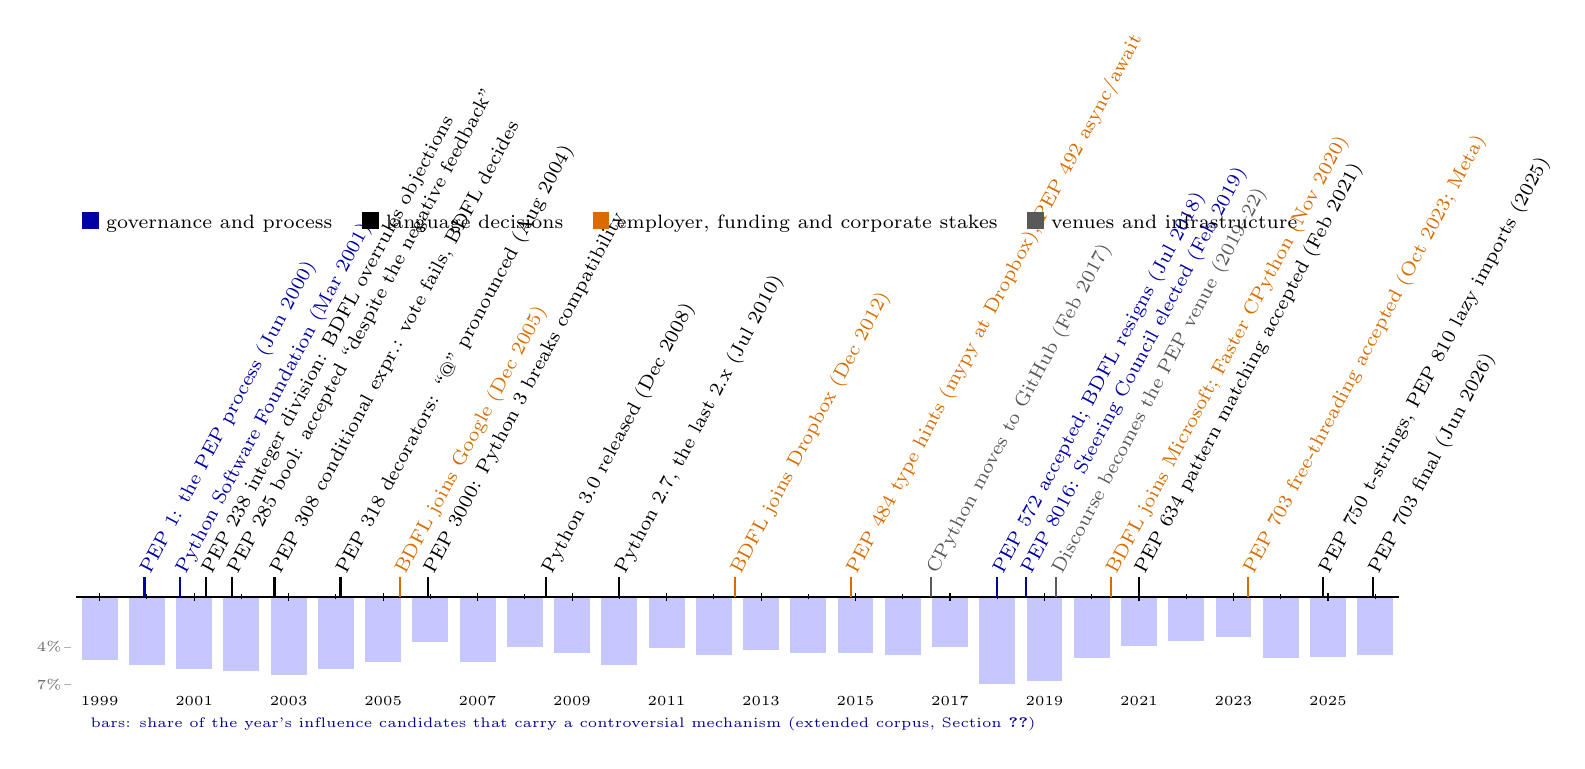
\begin{tikzpicture}[x=0.6cm, y=1cm, font=\scriptsize]
  % ---- yearly share of influence candidates that carry a controversial mechanism (extended corpus) ----
  \foreach \yr/\p in {1999/5.0, 2000/5.4, 2001/5.7, 2002/5.9, 2003/6.2, 2004/5.7, 2005/5.2, 2006/3.6, 2007/5.2,
                      2008/4.0, 2009/4.5, 2010/5.4, 2011/4.1, 2012/4.6, 2013/4.2, 2014/4.5, 2015/4.5, 2016/4.6,
                      2017/4.0, 2018/6.9, 2019/6.7, 2020/4.9, 2021/3.9, 2022/3.5, 2023/3.2, 2024/4.9, 2025/4.8, 2026/4.6} {
    \pgfmathsetmacro{\xl}{\yr-1999+0.12}
    \pgfmathsetmacro{\xr}{\yr-1999+0.88}
    \pgfmathsetmacro{\h}{-\p*0.16}
    \fill[blue!22] (\xl,0) rectangle (\xr,\h);
  }
  \draw[gray!60] (-0.25,-0.64) -- (-0.1,-0.64) node[left, text=gray!80!black, font=\tiny] {4\%};
  \draw[gray!60] (-0.25,-1.12) -- (-0.1,-1.12) node[left, text=gray!80!black, font=\tiny] {7\%};
  \node[anchor=west, text=blue!60!black, font=\tiny] at (0.1,-1.62) {bars: share of the year's influence candidates that carry a controversial mechanism (extended corpus, Section~\ref{sec:rq6})};
  % ---- axis and years ----
  \draw[thick] (0,0) -- (28,0);
  \foreach \yr in {1999,2001,...,2025} {
    \draw (\yr-1999+0.5,0.05) -- (\yr-1999+0.5,-0.05);
    \node[font=\tiny] at (\yr-1999+0.5,-1.33) {\yr};
  }
  \foreach \yr in {2000,2002,...,2026} { \draw (\yr-1999+0.5,0.03) -- (\yr-1999+0.5,-0.03); }
  % ---- landmark influences: x = fractional year, colour = kind ----
  \tikzset{gov/.style={blue!65!black}, lang/.style={black}, venue/.style={gray!70!black}, corp/.style={orange!85!black}}
  \foreach \x/\c/\t in {
    2000.45/gov/{PEP 1: the PEP process (Jun 2000)},
    2001.2/gov/{Python Software Foundation (Mar 2001)},
    2001.75/lang/{PEP 238 integer division: BDFL overrules objections},
    2002.3/lang/{PEP 285 bool: accepted ``despite the negative feedback''},
    2003.2/lang/{PEP 308 conditional expr.: vote fails, BDFL decides},
    2004.6/lang/{PEP 318 decorators: ``@'' pronounced (Aug 2004)},
    2005.85/corp/{BDFL joins Google (Dec 2005)},
    2006.45/lang/{PEP 3000: Python 3 breaks compatibility},
    2008.95/lang/{Python 3.0 released (Dec 2008)},
    2010.5/lang/{Python 2.7, the last 2.x (Jul 2010)},
    2012.95/corp/{BDFL joins Dropbox (Dec 2012)},
    2015.4/corp/{PEP 484 type hints (mypy at Dropbox), PEP 492 async/await},
    2017.1/venue/{CPython moves to GitHub (Feb 2017)},
    2018.5/gov/{PEP 572 accepted; BDFL resigns (Jul 2018)},
    2019.1/gov/{PEP 8016: Steering Council elected (Feb 2019)},
    2019.75/venue/{Discourse becomes the PEP venue (2019--22)},
    2020.9/corp/{BDFL joins Microsoft; Faster CPython (Nov 2020)},
    2021.5/lang/{PEP 634 pattern matching accepted (Feb 2021)},
    2023.8/corp/{PEP 703 free-threading accepted (Oct 2023; Meta)},
    2025.4/lang/{PEP 750 t-strings, PEP 810 lazy imports (2025)},
    2026.45/lang/{PEP 703 final (Jun 2026)}} {
    \draw[\c, thick] (\x-1999,0) -- (\x-1999,0.25);
    \node[\c, rotate=62, anchor=west, inner sep=1pt] at (\x-1999,0.27) {\t};
  }
  % ---- legend ----
  \node[anchor=south west, align=left, font=\scriptsize, inner sep=2pt] at (0,4.55) {%
    \textcolor{blue!65!black}{\rule{6pt}{6pt}} governance and process \quad
    \textcolor{black}{\rule{6pt}{6pt}} language decisions \quad
    \textcolor{orange!85!black}{\rule{6pt}{6pt}} employer, funding and corporate stakes \quad
    \textcolor{gray!70!black}{\rule{6pt}{6pt}} venues and infrastructure};
\end{tikzpicture}
\caption{Landmark influences on the Python project from the start of the corpus (python-dev, May 1999) to September 2026, above a corpus-derived measure of contestation: the share of each year's influence candidates that carry one of the seven controversial mechanisms (Section~\ref{sec:rq6}). Dates are from PEP headers, the \texttt{python/peps} history and python.org. Events were chosen because they changed who decides (governance), what the language is (each is the year's most discussed PEP in the corpus), who pays for the work, or where the discussion happens. The most contested years are 2003 (PEP~308's failed vote) and 2018--2019 (PEP~572 and the governance transition); the Steering Council's first years (2021--2023) are the least contested in the corpus.}
\label{fig:timeline}
\Description{A horizontal timeline from 1999 to 2026 with twenty-one labelled, colour-coded events rising from the axis at an angle, and a bar chart below the axis showing the yearly percentage of controversial influence candidates, peaking at about seven percent in 2018.}
\end{figure*}
\subsection{From Preferences to Influence}

Influence Miner complements these tools. While Preference Miner asks \emph{whose preferences matter}, Influence Miner asks \emph{how those preferences, arguments, roles and signals shape decisions}. Influence is not merely volume of participation. A participant who sends many emails may not influence a proposal, while another participant may send one message that reframes the problem, identifies a critical compatibility issue, invokes project authority or causes a proposal to be revised. Influence Miner therefore treats influence as a discursive, social, technical and governance phenomenon and aims to detect the sentence-level signals through which participants affect proposal trajectories.

\section{Research Questions}

The aim of this study is to develop and evaluate Influence Miner, a computational framework for mining influence mechanisms in OSS decision-making discussions.

\textbf{RQ1: What influence mechanisms appear in open source proposal discussions?} Which types of influence signals are used by participants, how frequently, and at which points of a proposal's life?

\textbf{RQ2: Which actors exercise influence, and through what mechanisms?} Is influence concentrated among formal leaders, core developers, proposal authors or the wider community, and do roles differ in the mechanisms they use?

\textbf{RQ3: How do influence mechanisms differ across governance models?} Within Python, do the discussions that continued after the 2018 governance transition differ from those under the BDFL model? (The Python--Bitcoin comparison is designed here but left for the next study.)

\textbf{RQ4: Do influence patterns align with proposal outcomes?} Are influence types and directions associated with acceptance, rejection, withdrawal or deferral?

\textbf{RQ5: How does Influence Miner complement existing decision-mining tools?}\  How much do influence signals overlap with the preference signals extracted by Preference Miner from the same corpus?

\textbf{RQ6: How much controversial influence is there, who exercises it, and did it change with governance?} How often do decisions by fiat, corporate interests, gatekeeping, exit threats, incivility, off-list agreements and procedural control appear, in whose messages, on which proposals, and how do their shares differ between the BDFL and Steering Council eras?

\section{Conceptualising Influence in OSS Decision-Making}

Influence is defined in this paper as a communicative or structural act that changes, constrains, legitimises, accelerates, blocks, reframes or redirects a proposal's decision trajectory. The unit of extraction in the prototype is the sentence; the unit of interpretation may be a message, a thread, an actor or a proposal trajectory.

Influence is different from preference. A preference expresses a position, such as support or opposition. Influence is the capacity of that position, argument, role or signal to affect the discussion or decision. A message may state a strong preference but fail to influence the proposal; conversely, a measured technical objection may substantially redirect the decision.

Influence is also different from sentiment. A message may be negative or frustrated without being influential, and a calm technical objection may be highly influential if it exposes a fundamental compatibility or security problem.

Influence is also different from rationale. A rationale explains why a decision was made. Influence Miner focuses on the mechanisms through which that rationale becomes accepted, contested or transformed during discussion. Influence Miner therefore sits between argument mining \cite{argumentMining}, rationale mining and social-network analysis: it connects what was said, who said it, when it was said and whether it appears to matter for the proposal trajectory.

\section{Influence Taxonomy}

Table~\ref{tab:taxonomy} summarises the taxonomy used by Influence Miner. It was developed from the DeMaP Miner research agenda, prior work on roles and rationale in Python, Bitcoin governance research \cite{thapa2021bitcoin}, and manual reading of PEP discussions. The thirteen types are not mutually exclusive: a sentence can carry several mechanisms at once, so the detector is multi-label. Table~\ref{tab:samples} in Section~\ref{sec:results} shows two sentences per mechanism as extracted by the tool.

\begin{table*}
\caption{Influence Miner taxonomy and indicative signals.}
\label{tab:taxonomy}
\begin{tabular}{p{0.16\textwidth}p{0.36\textwidth}p{0.40\textwidth}}
\toprule
\textbf{Influence type} & \textbf{Meaning} & \textbf{Indicative signals} \\
\midrule
Strategic & Shapes long-term direction, identity, philosophy or governance & future direction, project principles, Zen of Python, decentralisation, readability, simplicity \\
Operational & Shapes feasibility of implementation, maintenance, release, deployment, migration or testing & implementation burden, reference implementation, maintenance cost, release timing, documentation, backport \\
Functional & Shapes whether the proposed feature or protocol solves the intended problem & use case, edge case, API behaviour, semantics, syntax, alternative design, problem fit \\
Tactical & Shapes the immediate discussion trajectory & summarising, reframing, requesting evidence, compromise, deferral, closure, separate proposal \\
Authority & Uses formal or informal status to legitimise or block a decision & BDFL, delegate, steering council, BIP editor, core developer, pronouncement, veto \\
Compatibility & Shapes decisions through breaking-change and interoperability concerns & backward compatibility, existing code, Python 2/3, deprecation, old nodes, soft/hard fork \\
Security & Shapes decisions through safety, risk, attack, privacy or robustness concerns & vulnerability, attack surface, consensus failure, privacy, denial of service, crash \\
Standards & Uses existing standards, specifications or conventions as decision criteria & RFC, specification, PEP~8, protocol standard, compliance, convention \\
Ecosystem & Uses downstream adoption and ecosystem impact as decision criteria & PyPI, standard library, third-party packages, libraries, wallets, exchanges, miners, clients \\
Economic & Uses incentives, cost, funding, fees or business impact & cost, fees, funding, commercial pressure, developer time, block reward \\
Organizational & Uses companies, foundations, teams, working groups or institutions & PSF, company-backed maintainer, release team, committee, sponsor \\
Coalition & Uses collective alignment or repeated agreement as cumulative pressure & broad support, several developers, ``as others have said'', unanimous, seconded \\
User demand & Uses user needs, confusion, requests or adoption pressure & users want, beginners struggle, common request, pain point, widely used \\
\bottomrule
\end{tabular}
\end{table*}

\subsection{Strategic Influence}

Strategic influence refers to arguments that shape the long-term direction, identity, or governance of the project. It includes claims that a proposal is consistent or inconsistent with project philosophy, project values, or the future direction of the language, protocol, or ecosystem. In Python, such influence may invoke simplicity, readability, maintainability, or language identity. In Bitcoin, it may invoke decentralisation, consensus safety, censorship resistance, or protocol conservatism.

Examples of strategic influence include aligning a proposal with the project's long-term philosophy, arguing that a change affects the future direction of the language or protocol, invoking decentralisation or simplicity as a core value, and raising governance concerns about who has authority to decide. Strategic influence is especially important in proposals that affect language design, consensus rules, project governance, or ecosystem standards.

\subsection{Operational Influence}

Operational influence refers to arguments about implementation, maintenance, release management, tooling, deployment, testing, migration, and coordination. A proposal may be desirable in principle but difficult to implement, maintain, release, or deploy. Operational influence therefore determines whether a proposal can move from discussion to practical adoption.

Examples include arguing that a proposal is difficult to implement, showing that maintenance cost is too high, identifying release-timing constraints, discussing migration paths, pointing to lack of implementer capacity, or raising concerns about documentation, testing, and backward-compatibility management. Operational influence often determines whether a theoretically attractive proposal becomes practically feasible.

\subsection{Functional Influence}

Functional influence refers to arguments about whether the proposed feature, behaviour, protocol change, or API actually solves the intended problem. It is centred on design adequacy and problem-solution fit. Functional influence can support a proposal by demonstrating clear utility or block a proposal by showing that it does not solve the claimed problem.

Examples include demonstrating that the proposal does not meet user needs, showing that an alternative design solves the problem better, identifying edge cases, questioning whether the functionality is necessary, or arguing that the proposal introduces complexity disproportionate to its benefit. Functional influence is closely tied to technical evaluation and design quality.

\subsection{Tactical Influence}

Tactical influence refers to short-term moves in discussion that affect the direction of the debate. Tactical influence does not necessarily depend on formal authority; a participant can shape the trajectory of a thread by summarising disagreement, reframing a question, narrowing scope, requesting evidence, or proposing compromise.

Examples include summarising the state of discussion, reframing a disagreement, proposing compromise wording, redirecting the thread to a narrower issue, requesting evidence, calling for a decision, challenging an assumption, asking for a concrete implementation, or moving the discussion toward deferral, revision, or closure.

\subsection{Authority Influence}

Authority influence occurs when a participant's formal or informal status gives weight to a claim. Authority may come from governance position, maintainer status, long-term contribution, technical expertise, authorship, or decision-making role. In Python, this may involve the BDFL, Steering Council, PEP delegates, core developers, release managers, or recognised experts. In Bitcoin, it may involve BIP editors, Bitcoin Core maintainers, influential implementers, cryptographic experts, or long-standing community participants.

Examples include statements by a BDFL, steering council member, BDFL delegate, PEP delegate, core developer, BIP editor, maintainer, or recognised technical expert; references to previous decisions by authoritative actors; claims based on long-term project experience; and explicit pronouncements or veto-like interventions. Authority influence must be treated carefully. Influence Miner should not assume that all messages by high-status actors are influential; instead, it should detect whether their statements are taken up, deferred to, contested, or reflected in final outcomes.

\subsection{Compatibility Influence}

Compatibility influence refers to concerns about backward compatibility, interoperability, migration, deployment, or breaking changes. In mature OSS ecosystems, compatibility concerns can be decisive because even small changes may affect many downstream users, packages, clients, tools, nodes, or workflows.

Examples include claims such as a change will break existing code, old nodes must remain compatible, users cannot migrate easily, an API change conflicts with existing behaviour, or the ecosystem is not ready. Compatibility influence is likely to be especially important in Python language changes and Bitcoin consensus or protocol changes.

\subsection{Security Influence}

Security influence refers to arguments based on risk, vulnerability, attack surface, safety, consensus failure, abuse, privacy, or robustness. A security objection can be highly influential even if it is raised by a small number of participants, particularly when the proposal affects protocol safety or user assets.

Examples include identifying a new attack vector, questioning cryptographic assumptions, warning about unsafe implementation, raising denial-of-service, privacy, or consensus-safety issues, or arguing that the proposal reduces systemic resilience. In Bitcoin, security influence may be particularly important because protocol changes can affect funds, consensus, miners, nodes, wallets, and users.

\subsection{Standards Influence}

Standards influence refers to arguments that rely on existing standards, external specifications, interoperability norms, or cross-project conventions. A proposal may gain legitimacy because it aligns with an established standard, or it may be resisted because it conflicts with existing specifications.

Examples include aligning with internet standards, adopting widely used conventions, rejecting a proposal because it conflicts with a standard, or arguing that standardisation is needed for ecosystem coordination. Standards influence is particularly relevant when a project interacts with wider technical ecosystems, such as web standards, cryptographic standards, packaging standards, or protocol specifications.

\subsection{Ecosystem Influence}

Ecosystem influence refers to arguments based on the needs or behaviour of external projects, libraries, wallets, exchanges, miners, businesses, users, educators, or downstream communities. Ecosystem influence captures the reality that OSS decisions are not isolated within the core repository; adoption often requires coordination across a wider socio-technical network.

Examples include claims that major libraries already depend on an existing behaviour, wallet providers need a standard format, miners will not deploy a change, users are already relying on a pattern, or third-party implementations will be affected. Ecosystem influence is especially important in distributed projects where adoption requires coordination beyond the core repository.

\subsection{Economic Influence}

Economic influence refers to arguments based on incentives, cost, funding, market impact, transaction fees, business interests, or resource constraints. Economic influence is often explicit in blockchain settings, but it may also appear in language and infrastructure projects through maintenance cost, corporate adoption, and funded development.

Examples include deployment costs, miner incentives, maintenance funding, cost to users, commercial ecosystem pressure, and trade-offs between economic incentives and technical ideals. This category is likely to be more visible in Bitcoin than in Python, although Python may also show economic influence through corporate users, package maintainers, and institutional stakeholders.

\subsection{Organizational Influence}

Organizational influence refers to influence from companies, foundations, teams, institutions, or organised groups. It captures the fact that OSS decisions may be shaped not only by individual technical arguments but also by institutional resources, organised development capacity, sponsorship, foundation governance, or release-team priorities.

Examples include company-backed maintainers, foundation-level governance decisions, institutional support, release team priorities, organised working groups, and formal votes or committees. Organizational influence is not always explicit. It may appear through email domains, affiliations, funding acknowledgements, repeated coordination among participants, or the ability of an organization to implement and maintain a proposal.

\subsection{Coalition Influence}

Coalition influence occurs when multiple participants align around a position and create cumulative pressure. It differs from authority influence because the source of influence is not necessarily a single powerful actor but a visible convergence of multiple actors. Coalition influence may appear through repeated agreement, shared objections, mutual endorsement, or recurring references to a common concern.

Examples include several core developers converging on the same objection, users repeatedly raising the same problem, implementers agreeing that a proposal is not feasible, or miners, wallet developers, or downstream maintainers forming a visible block. Coalition influence can be detected through repeated agreement, quoting, endorsement, shared arguments, reply networks, and convergence of sentiment or stance.

\subsection{User-Demand Influence}

User-demand influence refers to arguments based on what users need, request, misunderstand, or struggle with. User-demand influence connects technical decisions to community needs and adoption pressure. It is especially important where proposals are justified by usability, learnability, adoption, error prevention, or common pain points.

Examples include claims such as users keep asking for this, this solves a common pain point, the current behaviour confuses beginners, this feature is needed by downstream users, or there is no real user demand. User-demand influence may support a proposal by demonstrating need, but it may also block a proposal if participants argue that demand is weak, misunderstood, or better addressed elsewhere.

\subsection{Controversial Mechanisms}
\label{sec:controversial}

The thirteen mechanisms above describe \emph{what} an argument appeals to. They say little about the forms of influence that the open source literature treats as contested: a leader deciding by fiat, a company steering a proposal towards its own product, a maintainer refusing to merge on the strength of ownership, a contributor threatening to leave or fork, hostility that silences opponents, agreements reached off-list, and process rules used to shut a discussion down. These are the episodes the software-engineering community remembers---the PEP~572 debate ended with the BDFL's resignation, and the Steering Council's constitution (PEP~13) is in part a response to them---so a tool that mines influence should be able to find them. Table~\ref{tab:controversial} defines seven further mechanisms, each grounded in a strand of the literature. They are detected with the same multi-label rules as the others, so a sentence can be both \emph{authority} and \emph{unilateral}, or \emph{organizational} and \emph{corporate interest}; the difference is that the thirteen base mechanisms classify the content of an argument, while the seven controversial ones classify the \emph{exercise of power} around it. Their cue lists are deliberately precision-oriented: most cues are first-person or explicit formulas (``I have decided'', ``my employer needs'', ``I will not merge'', ``I'll fork'', ``you clearly don't understand'', ``Guido and I agreed offline'', ``this belongs on python-ideas''), and the broad words only count near a disambiguating word (Appendix~\ref{app:rules}).

\begin{table*}[t]
\caption{Controversial influence mechanisms added to the taxonomy, with the literature that motivates each.}
\label{tab:controversial}
\small
\begin{tabular}{p{0.16\textwidth}p{0.47\textwidth}p{0.31\textwidth}}
\toprule
Mechanism & What it captures (representative cues) & Literature \\
\midrule
Unilateral & A decision announced by fiat rather than argued: ``I have decided'', ``end of discussion'', ``already merged'', ``not up for debate'', ``pull rank'', ``as BDFL'' & Benevolent-dictator governance and its legitimacy \cite{raymond1999, omahony2007} \\
Corporate interest & An employer, customer, funding or paid-time stake in the outcome: ``my employer needs'', ``our production code at \ldots'', ``we are paid to'', ``sponsored by'', ``conflict of interest'' & Firm participation in and capture of OSS projects \cite{dahlander2005, riehle2007, zhang2020} \\
Gatekeeping & Refusal grounded in ownership or veto position rather than in the merits: ``I will not merge'', ``as the maintainer'', ``over my dead body'', ``dead on arrival'', ``$-$1000'' & Gatekeepers and maintainer power \cite{ducheneaut2005, jensen2007} \\
Exit threat & Threats or announcements of exit, fork, withdrawal or burnout used as leverage: ``I'll fork'', ``I'm stepping down'', ``if this goes in I'm out'', ``withdraw the PEP'', ``permanent vacation'' & Exit versus voice \cite{hirschman1970}; forks \cite{robles2012, gamalielsson2014}; burnout \cite{raman2020} \\
Incivility & Ridicule, hostility and personal attacks that pressure rather than persuade: ``stupid'', ``you clearly don't understand'', ``bikeshedding'', ``ad hominem'', ``code of conduct'' & Incivility and toxicity in OSS discussion \cite{ferreira2021, squire2015, raman2020} \\
Backchannel & Decisions or agreements reached outside the public channel: ``offline'', ``in private'', ``at the sprint'', ``on IRC'', ``Guido and I agreed'', ``already been decided'', ``without discussion'' & Transparency of OSS decision-making \cite{schneider2016, omahony2007} \\
Procedural control & Process rules used to redirect or close a discussion: ``wrong list'', ``take it to python-ideas'', ``needs a sponsor'', ``already discussed'', ``PEP~1 says'', ``locking this thread'' & Proceduralisation of OSS governance \cite{delaat2007, fitzgerald2006} \\
\bottomrule
\end{tabular}
\end{table*}

\subsection{Internal and External Influence}

Orthogonally to the mechanism, Influence Miner records whether a signal is \emph{internal} (from or invoking the project's recognised governance and development structure) or \emph{external} (from or invoking users, downstream projects, companies, standards bodies, miners or market conditions), or \emph{mixed}, such as a core developer invoking user demand. This distinction is central to the planned Python--Bitcoin comparison: Python is expected to show stronger internal role-based influence, Bitcoin stronger ecosystem, economic, security and deployment-based influence.

\section{Influence Miner: Implementation}

Influence Miner is implemented as a Java extension of DeMaP Miner, following the design of Preference Miner, and reads the same MySQL corpus. Figure~\ref{fig:pipeline} shows the pipeline; this section describes what was built.

\begin{figure*}
  \centering
  \fbox{%
    \begin{minipage}{0.92\textwidth}
    \centering
    proposal-linked messages $\rightarrow$ automated-sender filter $\rightarrow$ identity and role resolution $\rightarrow$ text cleaning and sentence splitting $\rightarrow$ multi-label influence classification (type, direction, scope, target) $\rightarrow$ outcome and temporal features $\rightarrow$ heuristic scoring $\rightarrow$ candidate table $\rightarrow$ actor/proposal aggregation $\rightarrow$ CSV, annotation sample, report
    \end{minipage}}
  \caption{Influence Miner pipeline as implemented.}
  \Description{A flow diagram showing proposal-linked messages flowing through filtering, identity resolution, cleaning, classification, feature computation, scoring, storage, aggregation and reporting.}
  \label{fig:pipeline}
\end{figure*}

\subsection{Data Source and Message Filtering}

Messages are read from DeMaP Miner's \texttt{allmessages} table, which links mailing-list messages to PEP numbers by explicit references and subject matching \cite{sharma2022demap}. Column names are discovered at run time so that the same code can be pointed at a BIP database. Two classes of messages are excluded because they carry no human discussion: commit notifications from \texttt{python-checkins} (which embed entire PEP texts and would otherwise account for the majority of extracted sentences) and the bug- and patch-tracker robots (\texttt{report@bugs.python.org}, \texttt{noreply@sourceforge.net}). The exclusion lists are configurable. Messages that mention several PEPs appear once per PEP; duplicates within a PEP are collapsed.

\subsection{Identity and Role Resolution}

Actor identity is the person, not the address. The corpus provides a clustered display name and a pre-computed role per message; for the rows imported by a newer loader (chiefly 2017--2018, including the whole PEP~572 discussion) we found that the sender-address columns are shifted by one row---they belong to the \emph{next} message---while the clustered name and role agree with the raw ``From:'' header stored with the message body (Section~\ref{sec:threats}). Influence Miner detects these rows, keeps the name and role, and takes the address from the raw header. Roles are then resolved in layers: an optional manual, time-bounded mapping file; the role recorded on the message (BDFL, BDFL delegate, core developer, PEP editor, community member); proposal-specific roles from PEP metadata (proposal author, BDFL delegate); project-wide tables of core developers and PEP editors with their appointment dates; and well-known identities. Proposal-specific roles take precedence over project-wide ones, following the corpus's own convention, except that the BDFL keeps that role. Actors are keyed by the clustered name, which merges one person's several addresses.

\subsection{Text Cleaning and Sentence Splitting}

Each message body is cleaned before splitting: quoted lines, ``On \ldots wrote:'' introductions, forwarded header blocks, message-id and address debris, signature blocks, mailing-list footers, embedded PEP text attachments, code, diffs and tracebacks are removed, and URLs are replaced by a placeholder. Sentences are split on terminal punctuation with protection for abbreviations, version numbers and proposal references; short vote lines such as ``+1'' and ``$-$1'' are kept as sentences. A noise filter drops fragments shorter than three words, sentences longer than 120 words and lines that are mostly non-alphabetic. Cleaning is deliberately conservative: the research depends on real discussion content.

\subsection{Classification}

Four rule-based detectors label each sentence. The \emph{type} detector matches cue phrases for the twenty mechanisms (thirteen base, seven controversial) on word boundaries, accepts British and American spellings, requires disambiguating context for broad words (``break'' only near compatibility vocabulary, ``risk'' only near security vocabulary, ``team'' only near release or core vocabulary), and records the cue phrases that fired as \emph{evidence}, so that every label can be traced. The \emph{direction} detector is conservative: it classifies a sentence as supporting or blocking only on explicit stance phrases or votes, resolves negations (``I don't object'' is supporting, ``I can't support'' is blocking), treats a sentence with both supporting and blocking cues as ambiguous, demotes hedged sentences and questions, and otherwise assigns revising (revise, defer, clarify, narrow, alternative, compromise \ldots) or neutral. The \emph{scope} detector combines the author's role with actor words in the sentence; role alone never yields ``external''. The \emph{target} detector assigns governance, implementation, security, compatibility, ecosystem, users or proposal.

\subsection{Outcome, Temporal Features and Scoring}

The proposal outcome is resolved from the corpus's table of accepted and rejected PEPs and, for the remaining PEPs, from the PEP state history mined from the PEP repository log, normalised to accepted, rejected, withdrawn, deferred, final, active, superseded, draft, provisional or unknown, with the decision timestamp. From the decision date and the PEP creation date the tool computes the number of days between the message and the decision and a coarse decision phase (pre-draft, early discussion, active debate, revision, decision window, post-decision). A configurable governance split date (default 12~July~2018, when Guido van Rossum stepped down) assigns each message to the BDFL or post-BDFL era. Direction is compared with outcome to obtain an \emph{alignment} flag: supporting signals align with accepted, final or active proposals; blocking with rejected, withdrawn or deferred ones; revising with deferred, superseded, draft or provisional ones.

A transparent additive score combines the number of mechanisms detected, deontic and decision language, justification language, explicit reference to the proposal, a non-neutral direction, a resolved scope and target, the author's formal role, and proximity to the decision (only when the decision date is known and the message precedes it), with penalties for hedging and very short sentences. Sentences scoring at least 1.0 are stored as candidates with all labels, evidence cues, role, outcome and temporal features.

\subsection{Aggregation and Outputs}

A batch runner processes one proposal, a range or the whole corpus, continues after errors and logs per-proposal statistics. An aggregator populates per-actor and per-proposal summary tables and computes multi-label type distributions, direction, scope, role, phase and era distributions, type-by-outcome and type-by-era cross-tabulations and alignment counts. An exporter writes these as CSV files; a sampler exports a stratified annotation sheet (top-scored, random, per-type and per-outcome strata) with empty human-label columns; and a report generator writes a plain-text summary. All code, SQL and configuration are in the DeMaP Miner repository.

\subsection{Scoring in Detail}

The heuristic score is additive and every component is inspectable. A candidate starts at 0.8 for carrying at least one mechanism (+0.2 for a second, +0.2 for a third); +0.6 for deontic or decision language (\emph{should, must, need to, recommend, object, reject, accept, agree, insist, strongly, clearly}); +0.4 for justification language (\emph{because, therefore, for example, evidence, in practice, in my experience, shows that}); +0.5 for an explicit reference to the proposal (\emph{PEP~572, this change, this syntax, the spec}); +0.4 for a non-neutral direction; +0.2 for an internal or external scope and +0.4 for a mixed one; +0.3 for a recognised target; a role weight of 1.0 for the BDFL or Steering Council, 0.9 for a delegate, 0.8 for a core developer or release manager, 0.7 for a proposal author or PEP editor, 0.2 for a community member; +0.8, +0.5 or +0.2 when the message precedes a known decision by at most 7, 30 or 90 days; $-$0.2 for hedging (\emph{maybe, perhaps, not sure, I wonder}) and $-$0.3 for sentences shorter than six words unless they are votes. Unknown decision dates and post-decision messages add nothing, so proposals without a resolved decision are not boosted. The threshold of 1.0 keeps every sentence with a mechanism and at least one further signal; the annotation study will tell whether it should be raised.

\subsection{Tool Interfaces}

Influence Miner is delivered as a tab in both incarnations of the DeMaP Miner viewer, so that a candidate sentence is never more than one click away from the message it came from. In the Java desktop tool (Figure~\ref{fig:desktop}) the tab sits on the right-hand tabbed pane next to the existing \emph{Reasons}, \emph{InfluenceOfRoles} and \emph{SentimentOfMembers} tabs. Its controls filter by mechanism (including a \emph{Controversial (any of the 7)} option for the mechanisms of Section~\ref{sec:controversial}), direction, author role, governance era, minimum score and sort order; \emph{Load Influence Candidates} fills the results table of the viewer with the proposal's candidates (date, message id, author with role, mechanisms, direction, scope and target, sentence with its evidence cues, score) and a summary line gives the counts by mechanism and direction; \emph{Run Influence Miner for PEP} re-extracts the proposal in the background. Selecting a row loads the source message into the central viewer, exactly as for reason candidates, so that an analyst can read the sentence in its thread. In the web version (Figure~\ref{fig:web}), a Flask port of the same layout, the right-hand panel carries \emph{Reasons}, \emph{Preference Miner} and \emph{Influence Miner} tabs; the Influence Miner tab adds bar summaries of mechanisms and directions (controversial mechanisms highlighted in red), role and phase tags, a top-participants table and the candidate table with message links, and a separate overview page reports the corpus-wide distributions and the governance-era comparison of Section~\ref{sec:results}.3. Both interfaces read the same \texttt{influence\_candidates} table and can be pointed at either the original or the extended database.

\begin{figure*}[t]
\centering
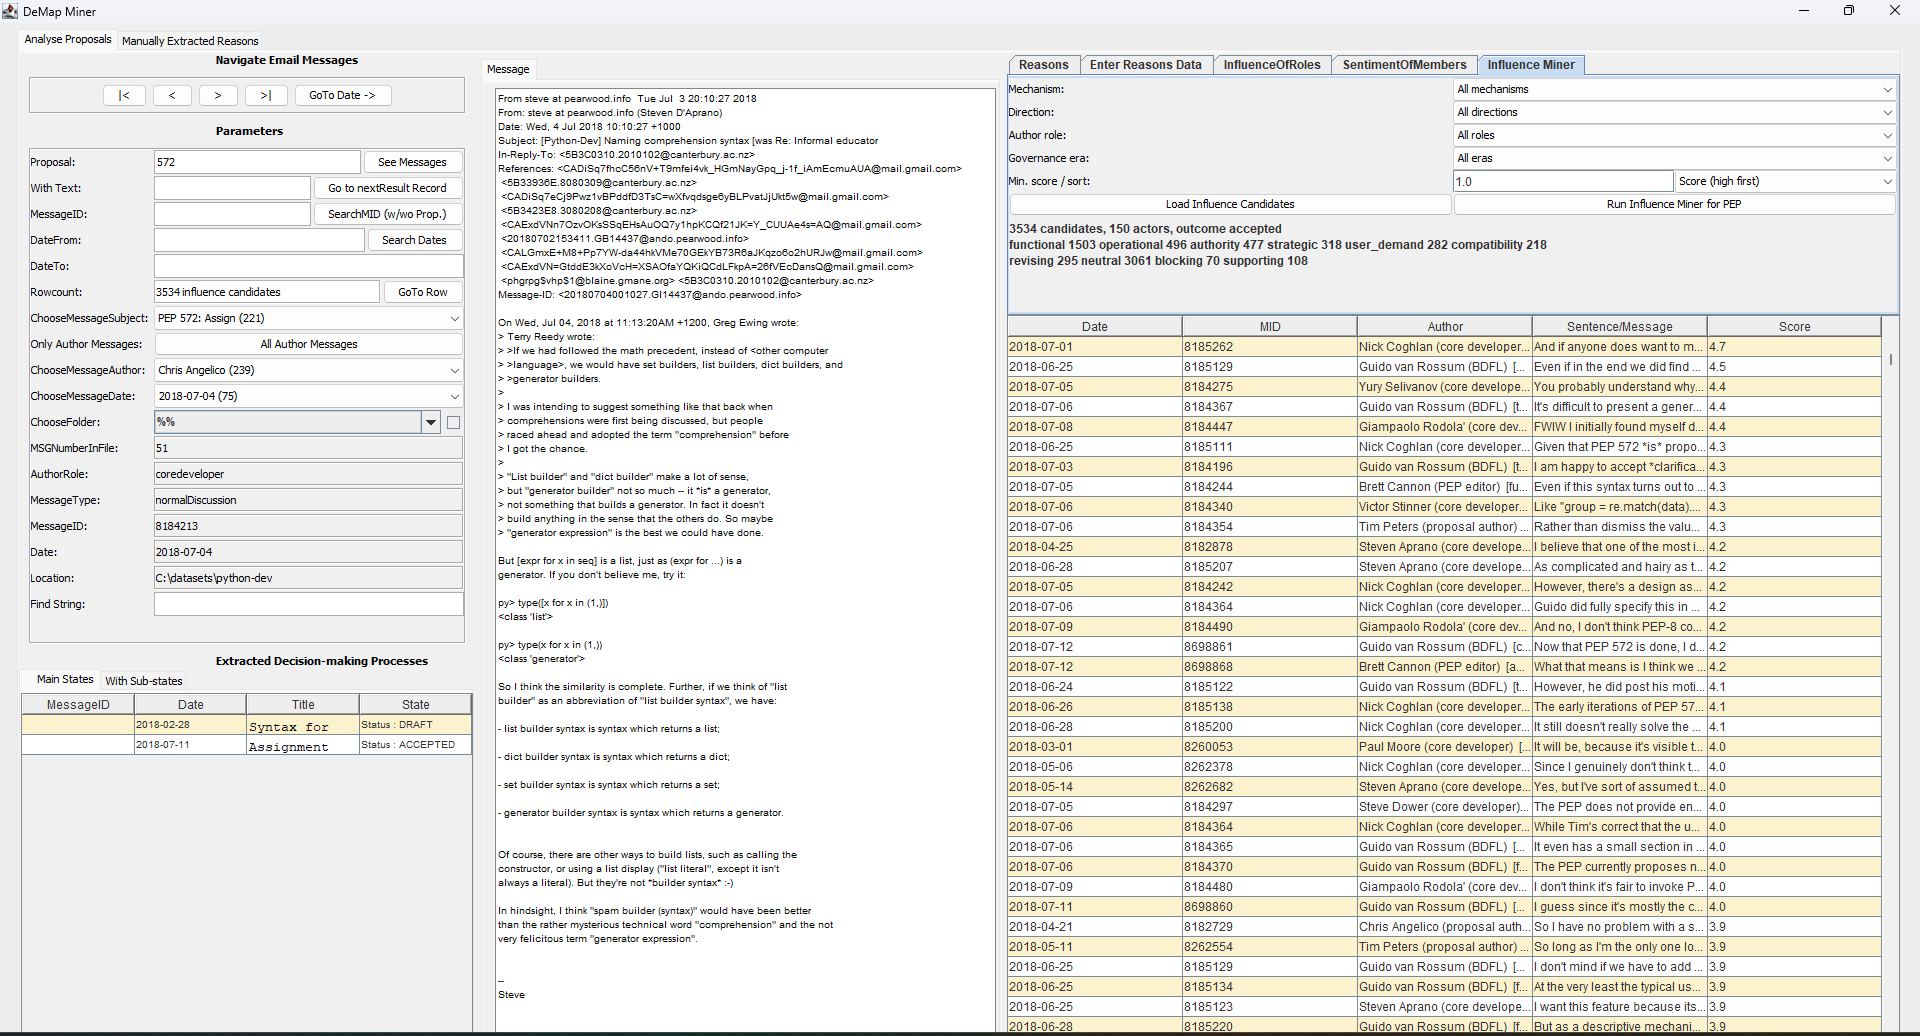
\includegraphics[width=\textwidth]{figures/fig_desktop_influence_tab_crop.png}
\caption{Influence Miner tab in the DeMaP Miner desktop tool (PEP~572, extended corpus). Right: filters, summary and the candidate table; centre: the message selected from the table; left: navigation, parameters and the PEP's state history.}
\Description{Screenshot of a Java Swing application with a maximised window: a left navigation panel, a central message viewer showing a python-dev e-mail, and a right panel whose "Influence Miner" tab shows filter drop-downs, a summary of 3,534 candidates and a table of candidate sentences with scores.}
\label{fig:desktop}
\end{figure*}

\begin{figure*}[t]
\centering
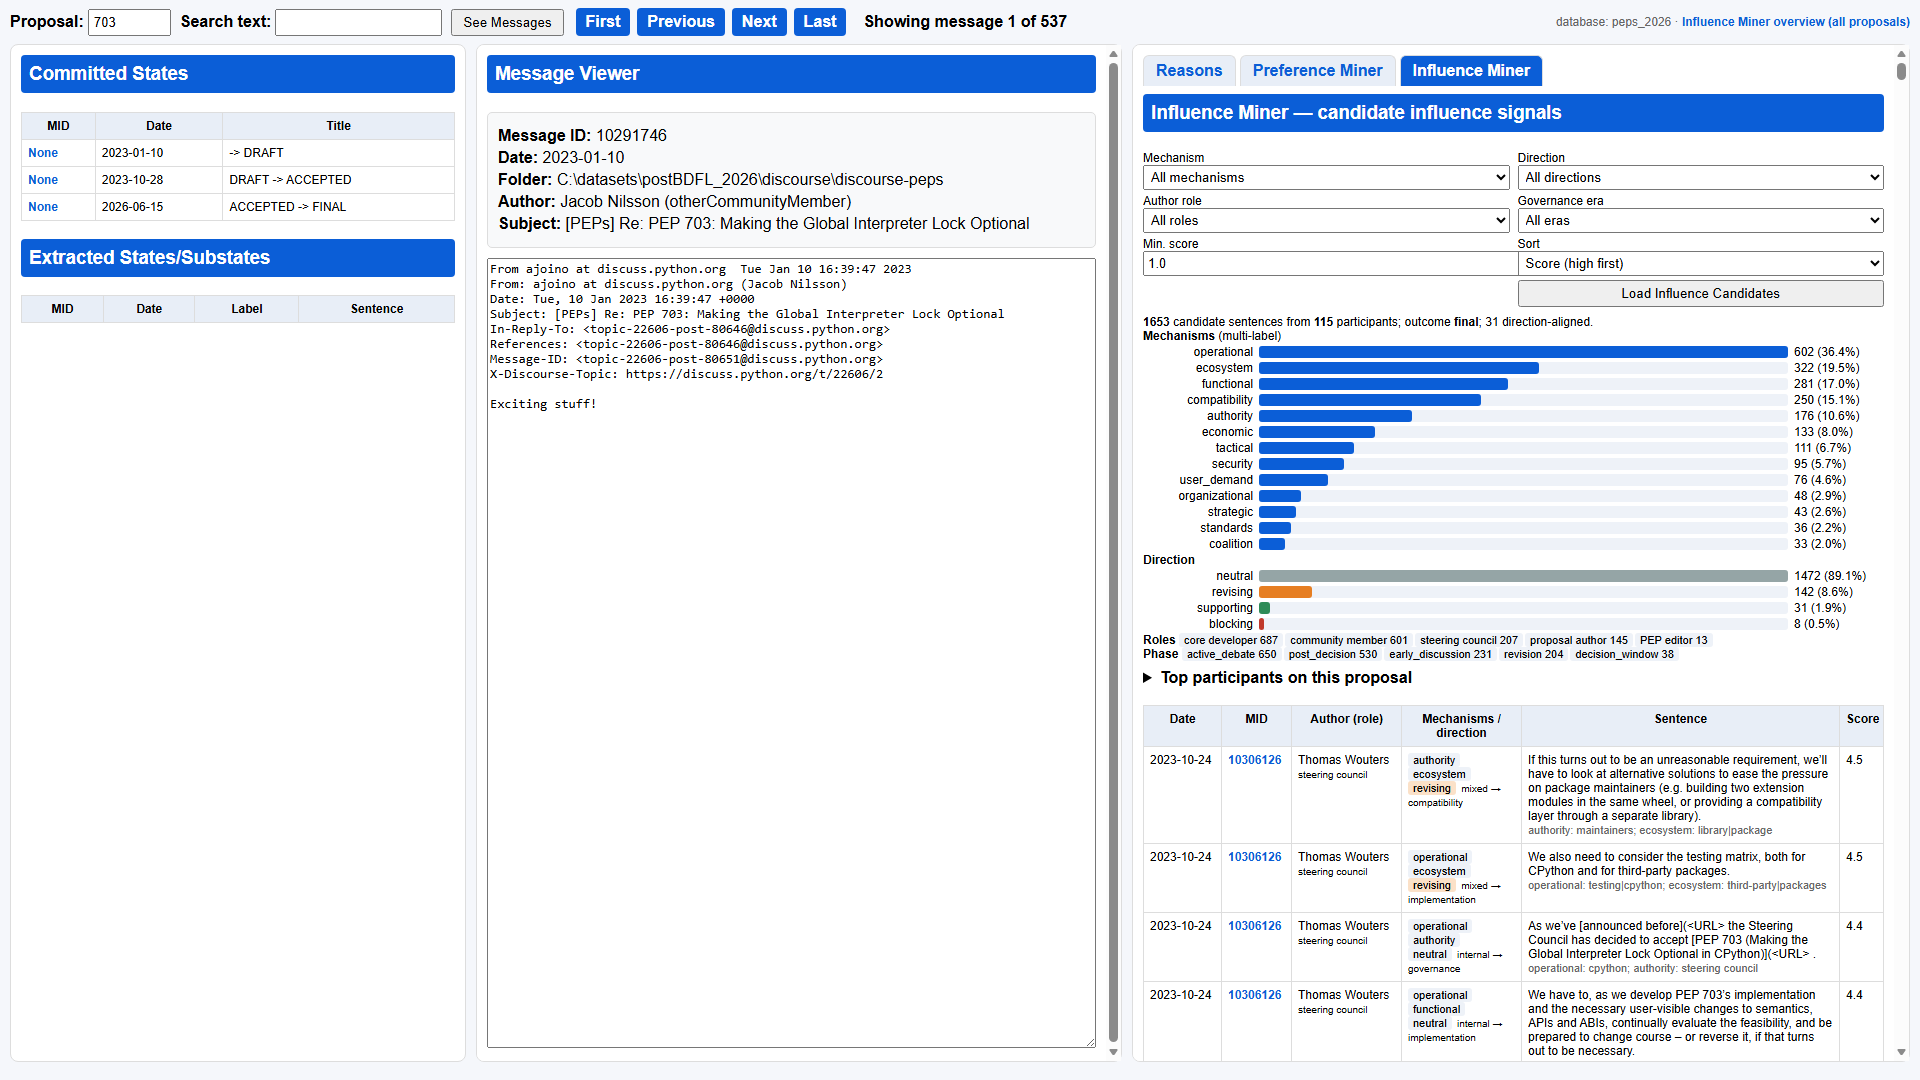
\includegraphics[width=\textwidth]{figures/fig_web_influence_tab_crop.png}
\caption{Influence Miner tab in the web version of DeMaP Miner (PEP~703, a Steering-Council-era proposal discussed on discuss.python.org). Left: the PEP's status history from the \texttt{python/peps} repository; centre: the selected Discourse post; right: filters, mechanism and direction bars, roles, phases and the candidate table.}
\Description{Screenshot of a browser window with three columns: committed states on the left, a message viewer in the middle, and on the right the Influence Miner tab with horizontal bars for thirteen mechanisms and four directions, role and phase tags, and the start of a candidate table.}
\label{fig:web}
\end{figure*}

\section{Study Design}

\subsection{Corpus}

The study uses the DeMaP Miner Python corpus \cite{sharma2022demap,sharma2024rationale}: messages from the python-dev, python-ideas, python-list, python-3000, distutils-sig, python-committers and python-announce lists, linked to PEP numbers, spanning May~1999 to November~2018. Table~\ref{tab:corpus} summarises the run. Of the 109,046 PEP-linked message rows, 28,412 were excluded as automated senders, leaving 80,634 human-authored messages across 523 PEPs. Cleaning and splitting produced 999,943 sentences, of which 199,409 (19.9\%) carried at least one influence mechanism and scored above the threshold. The run took 31~minutes on a laptop.

\begin{table}[t]
\caption{Corpus and extraction summary.}
\label{tab:corpus}
\begin{tabular}{lr}
\toprule
PEPs with linked messages & 523 \\
PEP-linked message rows & 109,046 \\
\quad automated (commit/tracker) rows excluded & 28,412 \\
\quad human-authored messages processed & 80,634 \\
Sentences after cleaning & 999,943 \\
Influence candidate sentences stored & 199,409 \\
PEPs with at least one candidate & 508 \\
Distinct participants (actors) & 2,376 \\
Period covered & 1999-05 to 2018-11 \\
\bottomrule
\end{tabular}
\end{table}

Outcomes were resolved for 479 of the 523 PEPs: 151 accepted, 94 rejected, 83 final, 42 withdrawn, 34 draft, 30 deferred, 25 active and 5 superseded; 44 PEPs (1,343 candidates, 0.7\%) have no recorded state. Candidates on accepted or final proposals make up 64\% of the corpus, rejected 12\%, withdrawn 7\% and deferred 4\%.


\subsection{Extending the Corpus to the Steering Council Era}
\label{sec:extension}

The DeMaP Miner corpus ends in November~2018, four months after the governance transition, so a comparison of eras needed new data. Python's discussions had meanwhile moved twice: the mailing lists migrated from Mailman~2 to Mailman~3 in mid-2019, and proposal discussion moved from python-dev and python-ideas to the Discourse forum at discuss.python.org, which PEP~1 now names as the default venue. The extension therefore had three sources, summarised in Table~\ref{tab:sources}, and was designed so that every new message passes through DeMaP Miner's own reader and PEP-linking code unchanged.

\begin{table}[t]
\caption{Sources of the corpus extension (November~2018 to September~2026).}
\label{tab:sources}
\footnotesize
\setlength{\tabcolsep}{3.5pt}
\resizebox{\columnwidth}{!}{%
\begin{tabular}{llrr}
\toprule
Source & Period & Messages & PEP-linked \\
\midrule
python-dev (Mailman~2/3) & 2018-11 -- 2023-11 & 14,554 & 6,918 \\
python-ideas (Mailman~2/3) & 2018-11 -- 2024-06 & 20,438 & 3,873 \\
python-committers (Mailman~2/3) & 2018-11 -- 2023-07 & 1,925 & 744 \\
python-list & 2018-11 -- 2025-05 & 25,565 & 1,175 \\
python-checkins & 2018-11 -- 2023-08 & 27,658 & 1,715 \\
python-bugs-list & 2018-11 -- 2022-04 & 133,818 & 5,219 \\
Discourse: PEPs (223 topics) & 2019-03 -- 2026-09 & 15,180 & 14,892 \\
Discourse: Ideas (2,041 topics) & 2018-02 -- 2026-09 & 34,293 & 2,849 \\
Discourse: Core Dev.\ (952 topics) & 2019-10 -- 2026-09 & 11,880 & 1,991 \\
Discourse: Committers (469 topics) & 2018-09 -- 2026-09 & 3,768 & 1,572 \\
\midrule
Total & & 289,079 & 40,948 \\
\bottomrule
\end{tabular}}
\end{table}

\paragraph{Mailing lists.} Mailman~2 monthly archives were downloaded from mail.python.org for the six lists the original study used; they are the same text format the reader was written for. From July~2019 the core lists exist only in Mailman~3, whose HyperKitty archiver exports a month at a time as an mbox with MIME bodies, folded headers and RFC~2047 encoded words. A converter, \texttt{HyperKittyMbox\allowbreak ToPipermail}, unfolds headers, takes the first \texttt{text/plain} part (falling back to tag-stripped HTML), decodes quoted-printable and base64, and rewrites each message in the Mailman~2 layout; on an overlapping month it produced exactly the same number of messages as the Mailman~2 archive. python-dev and python-ideas fell silent in 2023--2024 as discussion completed its move to Discourse.

\paragraph{Discourse.} discuss.python.org exposes a JSON API. A crawler (\texttt{DiscourseToPipermail}) enumerates the topics of a category and fetches every post with its raw Markdown, then writes each post as a pipermail-style message: the Discourse username stands in for the address (\texttt{user at discuss.python.org}), the display name is kept, the topic title becomes the subject, the topic's first post becomes the \texttt{In-Reply-To} parent of every later post (or the quoted post when a reply is explicit), and \texttt{[quote]} blocks become quoted lines so that the existing quote removal applies. Two properties of the site had to be worked around: category listings stop after a few hundred topics in any sort order, so topics were enumerated with the search API restricted to topic-opening posts (\texttt{in:first}) in half-month windows; and anonymous search is rate-limited at roughly fifteen requests a minute, and requests that ask for \texttt{application/json} explicitly are throttled harder than plain ones. The four categories that correspond to the old lists---PEPs, Ideas, Core Development and Committers---yielded 3,685 topics and 63,714 posts. The PEPs category is the main venue of the Steering Council era: almost every post in it links to a PEP.

\paragraph{PEP metadata and state history.} Instead of scraping python.org as the original tool did, the \texttt{python/peps} repository was cloned and its git history parsed: every commit that changes a \texttt{Status:} line yields a (PEP, from, to, timestamp) record, giving 1,859 status changes for 739 PEPs from 2000 to September~2026. On the PEPs both tables cover, the regenerated history agrees exactly with the state table of the original study (for example PEP~572: draft 28~Feb~2018, accepted 11~July~2018), and it adds the later transitions (PEP~572 final in November~2022; PEP~703 draft January~2023, accepted October~2023, final June~2026). PEP headers supplied title, authors, type, creation date, delegate, sponsor and the \texttt{Discussions-To} link for the 261 PEPs the original metadata table lacked.

\paragraph{Roles.} The corpus's role vocabulary (BDFL, BDFL delegate, core developer, PEP editor, proposal author, community member) was extended with \emph{steering council}, assigned by name and term from the election results recorded in PEPs 8100--8107 (2019--2026). Core-developer status was refreshed from the devguide's core-team roster, which lists join and leave dates for 210 people, and matched on full name and on first plus last name (the roster spells out middle names). Proposal author and delegate remain proposal-specific and come from the PEP headers.

\paragraph{Reading and post-reading.} The reader assigned message ids continuing after the corpus's maximum, and a post-reading script derived the sender address and name from the raw \texttt{From:} header of each message, keyed by message id, so that the row shift described in Section~\ref{sec:dataquality} cannot recur; cluster names were reused from the original corpus where the address was known. The reading of 289,079 messages took about an hour; the Influence Miner run over the extended corpus of 780 PEPs and 114,388 human-authored messages took 37~minutes and produced 291,100 candidates from 3,613 participants, of which 100,778 candidates on 579 PEPs fall after the governance split.

\subsection{Analysis}

RQ1 is answered by the multi-label type distribution, its profile across decision phases and the timing of signals relative to the decision. RQ2 uses the role distribution, actor-level aggregates and direction by role. RQ3 compares mechanism, role, direction and alignment distributions of BDFL-era and Steering-Council-era candidates on the extended corpus, and the mechanism mix of the decision-makers of each era (the BDFL; Steering Council members during their terms). RQ4 compares type distributions across outcomes, per-proposal averages, and direction--outcome alignment against the base rate. RQ5 compares influence sentences with the 12,690 sentences stored by Preference Miner for the same PEPs after normalising whitespace and punctuation. RQ6 uses the seven controversial mechanisms: their frequency, their share within roles, eras, venues, outcomes and decision phases, the proposals in which they concentrate, and example sentences. All statistics are descriptive; no causal claim is made.

\section{Results}
\label{sec:results}

\subsection{RQ1: Influence Mechanisms}

Table~\ref{tab:rq1} shows how often each mechanism occurs among the 199,409 candidates. Because a sentence can carry several mechanisms, the percentages sum to more than 100 (on average 1.27 mechanisms per candidate). Four mechanisms dominate: operational (27.1\%), functional (25.2\%), ecosystem (19.9\%) and compatibility (14.4\%). Standards signals (9.8\%) are inflated by the many references to PEP~8 and PEP~257 as style standards. Authority signals appear in 7.1\% of candidates, strategic signals in 5.0\% and tactical moves in 4.9\%. The mechanisms that the Bitcoin literature emphasises---economic (2.3\%), coalition (2.0\%) and security (2.8\%)---are rare in Python's language-design discussions, as expected.

\begin{table}[t]
\caption{RQ1: influence mechanisms in 199,409 candidate sentences (multi-label).}
\label{tab:rq1}
\begin{tabular}{lrr}
\toprule
Mechanism & Candidates & \% of candidates \\
\midrule
Operational & 54,098 & 27.1 \\
Functional & 50,233 & 25.2 \\
Ecosystem & 39,593 & 19.9 \\
Compatibility & 28,656 & 14.4 \\
Standards & 19,631 & 9.8 \\
Authority & 14,078 & 7.1 \\
Strategic & 10,018 & 5.0 \\
Tactical & 9,780 & 4.9 \\
User demand & 7,193 & 3.6 \\
Organizational & 5,914 & 3.0 \\
Security & 5,529 & 2.8 \\
Economic & 4,555 & 2.3 \\
Coalition & 4,010 & 2.0 \\
\bottomrule
\end{tabular}
\end{table}

Table~\ref{tab:samples} shows two sentences per mechanism as the tool extracted and labelled them, chosen among high-scoring candidates with different roles and directions. They illustrate what the labels mean in practice: the BDFL closing a debate (``I heard all the feedback \ldots and have decided''), a delegate asking whether a PEP is ready for pronouncement, a core developer proposing that a contentious part be deferred to a separate PEP, a proposal author conceding a cost, a community member reporting classroom evidence.

\begin{table*}
\caption{Sample statements per influence mechanism, as extracted and labelled by Influence Miner (role and direction as assigned by the tool; ``rev.'' = revising).}
\label{tab:samples}
\small
\begin{tabular}{p{0.095\textwidth}p{0.045\textwidth}p{0.125\textwidth}p{0.66\textwidth}}
\toprule
\textbf{Mechanism} & \textbf{Dir.} & \textbf{Role, PEP} & \textbf{Sentence} \\
\midrule
Strategic & supp. & core dev., 492 & In principle, I support the PEP, on the basis that working towards better coroutine/async support in Python seems worthwhile to me. \\
 & block. & core dev., 20 & I'm not putting either version forward as paragons of Pythonic code, but honestly, they're not so awful that we should reject this PEP because of the risk that somebody will do this. \\
\midrule
Operational & supp. & BDFL, 3147 & I'm fine with the implementation going in and the PEP being marked as accepted as long as you get to the clarifications I suggest below soon after. \\
 & rev. & BDFL, 365 & Unless I find someone besides Phillip who is interested in having this included and is willing to help maintain it, I don't really think it would be wise to accept this into the standard library. \\
\midrule
Functional & supp. & BDFL, 435 & I heard all the feedback, took into account my own thoughts, and have decided that we should go ahead with this syntax and the \_getframe() hack. \\
 & rev. & BDFL, 525 & The provisional status is because this is a big project and it's likely that we'll need to tweak some small aspect of the API once the code is in, even after 3.6.0 is out. \\
\midrule
Tactical & rev. & core dev., 565 & IMHO the core of the PEP 565 is to propose a compromise to separate ``own code'' and ``external code'' (cannot be modified). \\
 & rev. & core dev., 470 & Instead, the PEP should highlight this compromise and defer it to a separate PEP. \\
\midrule
Authority & rev. & BDFL, 441 & So is the PEP ready for pronouncement or should there be more discussion? \\
 & neutral & BDFL, 380 & I just can't get used to this aspect of PEP 3152, so I'm rejecting it. Sorry Greg, but that's the end. \\
\midrule
Compatibility & supp. & core dev., 476 & So while I agree with the intent of PEP 476, and like the suggested end state, I'm back to thinking that the transition plan for existing corporate users needs more work before it can be accepted. \\
 & block. & author, 438 & However, I think PEP470 needs to achieve stronger backward compatibility for end-users because, as is typical for the 99\%, they like to see change but hate to be forced to change themselves. \\
\midrule
Security & rev. & author, 438 & If projects host on HTTP instead of HTTPS, users are vulnerable against MITM attacks whereas PEP438f provides a checksummed link from PyPI which cannot be easily man-in-the-middled. \\
 & rev. & author, 504 & The PEP would then stay deferred until someone actually did the research and demonstrated a practical attack. \\
\midrule
Standards & supp. & core dev., 371 & I agree that the threading and the pyprocessing APIs should be PEP 8 compliant, but I think 2 APIs is almost worse than one wrong one. \\
 & neutral & delegate, 427 & The compatibility tag spec itself looks fine to me, so with the above clarifications, I will accept the PEP. \\
\midrule
Ecosystem & supp. & core dev., 470 & Since PyPI is legally run by the PSF, the PSF board will have to approve the new terms. \\
 & rev. & BDFL, 365 & If its inclusion is really meant just as a bootstrap to simplify installing other package management solutions, as the PEP claims, I would prefer to see something with a much smaller footprint. \\
\midrule
Economic & neutral & author, 441 & IMO, the costs aren't worth the benefits, and I'd like to remove this proposal and simply document that applications packed up with pyzaa need to be tested to ensure they work from a zipfile. \\
 & rev. & community, 285 & Probably `should', at least---yet more work (`transitional', to be sure), and so yet another cost of the PEP's adoption. \\
\midrule
Organizational & neutral & BDFL, 3149 & That's about as large a committee I'd be comfortable to appoint for any specific PEP. \\
 & rev. & core dev., 466 & Presumably the need for such enhancements is there (or there'd be no need for this PEP) so is it simply that companies like Red Hat don't know that they have this option? \\
\midrule
Coalition & supp. & BDFL, 3154 & Assuming Tim doesn't object (hi Tim!) I think this PEP is fine to accept---all the ideas sound good, and I agree with moving to support 8-byte sizes and framing. \\
 & neutral & BDFL, 363 & This seems to be the overwhelming feedback at this point, so I'm withdrawing my support for the proposal. \\
\midrule
User demand & rev. & core dev., 362 & Since this will be an error that beginners see (frequently), I suggest ArgumentError is more friendly than BindError. \\
 & rev. & community, 572 & I've only had the chance to test the proposal on $\sim$20 students so far, but I'd like the chance to gather more data for your consideration before the PEP is accepted or rejected. \\
\bottomrule
\end{tabular}
\end{table*}

Direction is neutral for 88.1\% of candidates; 8.6\% are revising, 2.0\% supporting and 1.3\% blocking. This is by design: the detector only commits to a direction on explicit cues, so the non-neutral 11.9\% are high-precision signals for later analysis. Scope is internal for 61.7\%, mixed for 4.5\%, external for 2.5\% and unresolved for 31.3\%.

\paragraph{When influence is exercised.} Temporally, 33.3\% of candidates were written \emph{after} the recorded decision (implementation and follow-up discussion), 33.1\% during active debate, 9.5\% in the first month after the PEP was created, 8.1\% in the two weeks before the decision and 6.2\% in the preceding revision window. Figure~\ref{fig:timeline} shows the volume of influence signals per two-week bin relative to the decision date: signalling builds up over the preceding quarter and peaks sharply in the two weeks before the decision (13,702 candidates) and the two weeks after it (9,022), then falls back within a month to the pre-decision level. Sentences with an explicit stance follow the same curve (604 in the last two weeks). The decision moment recorded in the PEP repository is therefore also the moment of maximum argumentative activity in the mailing lists, which supports the use of the decision date to define the ``decision window'' phase.

\begin{figure}[t]
\centering
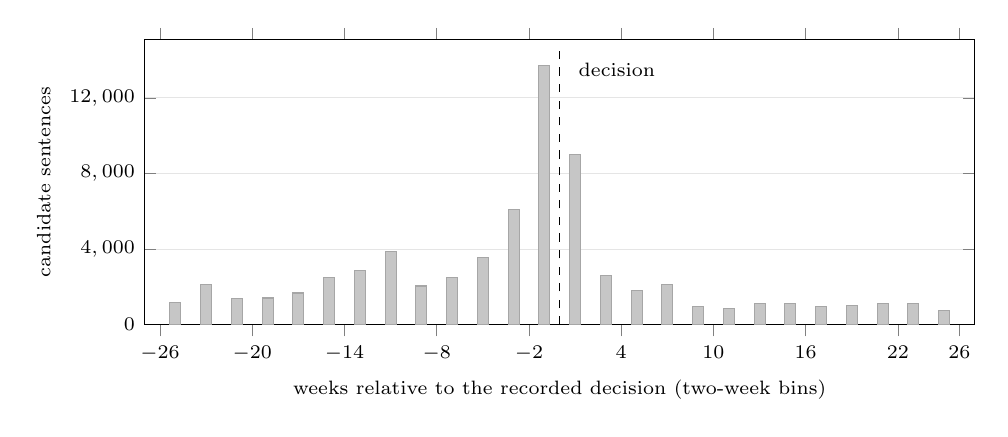
\begin{tikzpicture}
\begin{axis}[
  width=\columnwidth, height=5.2cm,
  ybar, bar width=4pt,
  xlabel={weeks relative to the recorded decision (two-week bins)},
  ylabel={candidate sentences},
  xmin=-27, xmax=27, ymin=0,
  xtick={-26,-20,-14,-8,-2,4,10,16,22,26},
  scaled y ticks=false,
  ytick={0,4000,8000,12000},
  yticklabel style={/pgf/number format/fixed, /pgf/number format/1000 sep={,}},
  tick label style={font=\scriptsize}, label style={font=\scriptsize},
  enlarge x limits=false,
  ymajorgrids, grid style={gray!20},
]
\addplot[fill=gray!45, draw=gray!70] coordinates {
(-25,1187) (-23,2130) (-21,1362) (-19,1413) (-17,1677) (-15,2486) (-13,2887) (-11,3883) (-9,2045) (-7,2512) (-5,3559) (-3,6115) (-1,13702)
(1,9022) (3,2618) (5,1788) (7,2114) (9,947) (11,837) (13,1138) (15,1124) (17,975) (19,1025) (21,1108) (23,1098) (25,758) };
\draw[dashed] (axis cs:0,0) -- (axis cs:0,14500);
\node[font=\scriptsize, anchor=west] at (axis cs:0.6,13500) {decision};
\end{axis}
\end{tikzpicture}
\caption{Influence candidates per two-week bin relative to the proposal's recorded decision date (69,510 candidates within $\pm$26 weeks of a known decision).}
\Description{Bar chart of candidate sentences per two-week bin from 26 weeks before to 26 weeks after the decision; volume rises slowly, peaks at 13,702 in the two weeks before the decision and 9,022 in the two weeks after, then drops to around one to two thousand per bin.}
\label{fig:timeline}
\end{figure}

\paragraph{Which mechanisms when.} Figure~\ref{fig:phases} profiles the mechanisms across four phases of a proposal's life. Functional arguments are most frequent early (30.1\% of early-discussion candidates) and again in the decision window (29.0\%), when the community is deciding whether the proposal solves the right problem; strategic arguments follow the same shape (6.8\% early, 6.2\% in the window, 3.9\% after). Compatibility (11.1\% $\rightarrow$ 17.8\%) and operational arguments (24.0\% $\rightarrow$ 30.2\%) rise steadily and dominate \emph{after} the decision, when accepted proposals are implemented and their effects on existing code are discovered. Authority, tactical and coalition signals are flat or fall after the decision. Influence Miner thus recovers the expected lifecycle of a design decision from the text alone: what-and-why arguments first, how-and-what-breaks arguments later.

\begin{figure*}[t]
\centering
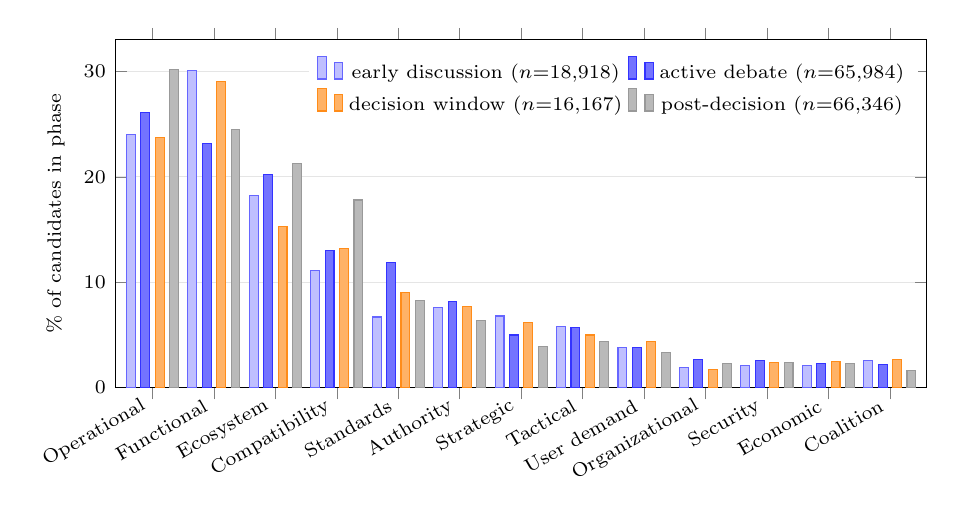
\begin{tikzpicture}
\begin{axis}[
  width=0.98\textwidth, height=6cm,
  ybar, bar width=3.2pt,
  ylabel={\% of candidates in phase},
  ymin=0, ymax=33,
  symbolic x coords={Operational,Functional,Ecosystem,Compatibility,Standards,Authority,Strategic,Tactical,User demand,Organizational,Security,Economic,Coalition},
  xtick=data, x tick label style={rotate=30, anchor=east, font=\scriptsize},
  tick label style={font=\scriptsize}, label style={font=\scriptsize},
  enlarge x limits=0.05,
  legend style={font=\scriptsize, at={(0.99,0.97)}, anchor=north east, legend columns=2, draw=none, fill=white},
  ymajorgrids, grid style={gray!20},
]
\addplot[fill=blue!25, draw=blue!60] coordinates {(Operational,24.0) (Functional,30.1) (Ecosystem,18.2) (Compatibility,11.1) (Standards,6.7) (Authority,7.6) (Strategic,6.8) (Tactical,5.8) (User demand,3.8) (Organizational,1.9) (Security,2.1) (Economic,2.1) (Coalition,2.6)};
\addplot[fill=blue!55, draw=blue!80] coordinates {(Operational,26.1) (Functional,23.2) (Ecosystem,20.2) (Compatibility,13.0) (Standards,11.9) (Authority,8.2) (Strategic,5.0) (Tactical,5.7) (User demand,3.8) (Organizational,2.7) (Security,2.6) (Economic,2.3) (Coalition,2.2)};
\addplot[fill=orange!60, draw=orange!90] coordinates {(Operational,23.7) (Functional,29.0) (Ecosystem,15.3) (Compatibility,13.2) (Standards,9.0) (Authority,7.7) (Strategic,6.2) (Tactical,5.0) (User demand,4.4) (Organizational,1.7) (Security,2.4) (Economic,2.5) (Coalition,2.7)};
\addplot[fill=gray!55, draw=gray!80] coordinates {(Operational,30.2) (Functional,24.5) (Ecosystem,21.3) (Compatibility,17.8) (Standards,8.3) (Authority,6.4) (Strategic,3.9) (Tactical,4.4) (User demand,3.3) (Organizational,2.3) (Security,2.4) (Economic,2.3) (Coalition,1.6)};
\legend{{early discussion ($n$=18{,}918)},{active debate ($n$=65{,}984)},{decision window ($n$=16{,}167)},{post-decision ($n$=66{,}346)}}
\end{axis}
\end{tikzpicture}
\caption{Mechanism profile by decision phase (share of the phase's candidates carrying each mechanism; multi-label, so bars within a phase sum to more than 100\%).}
\Description{Grouped bar chart with thirteen mechanisms on the x axis and four bars per mechanism for early discussion, active debate, decision window and post-decision. Functional and strategic bars are highest early and in the decision window; compatibility and operational bars are highest after the decision.}
\label{fig:phases}
\end{figure*}

\subsection{RQ2: Who Exercises Influence}

Table~\ref{tab:rq2} breaks candidates down by the author's role on the proposal in question. Core developers produce 25.6\% of candidates and community members 36.6\%, but the 138 core developers identified are far fewer than the 2,162 community members, so influence signalling per person is much denser among core developers. Proposal authors contribute 15.7\% and the BDFL alone 10.9\% of all candidates (21,793 sentences across 464 PEPs). PEP editors (9.4\%) and BDFL delegates (1.7\%) are small groups with high per-person volume.

\begin{table}[t]
\caption{RQ2: candidates and participants by role. Roles are proposal-specific; a person is counted under the role they held most often.}
\label{tab:rq2}
\begin{tabular}{lrrr}
\toprule
Role & Candidates & \% & Participants \\
\midrule
Community member & 72,976 & 36.6 & 2,162 \\
Core developer & 51,026 & 25.6 & 138 \\
Proposal author & 31,369 & 15.7 & 52 \\
BDFL & 21,793 & 10.9 & 1 \\
PEP editor & 18,656 & 9.4 & 8 \\
BDFL delegate & 3,431 & 1.7 & 1 \\
Unknown & 158 & 0.1 & 12 \\
\bottomrule
\end{tabular}
\end{table}

The fifteen most active participants account for 52\% of all candidates: Guido van Rossum (24,336 candidates, 464 PEPs), Brett Cannon (16,342; 285), Nick Coghlan (16,040; 332), Steven Bethard (7,270; 95), Phillip Eby (5,202; 108), Victor Stinner (4,932; 142), Donald Stufft (4,188; 67), Paul Moore (4,186; 178), Ned Deily (3,671; 73), Steven D'Aprano (3,528; 151), Tony Meyer, Yury Selivanov, Barry Warsaw, Martin von L\"owis and Tim Peters. Their mechanism mix is remarkably uniform---operational, functional and ecosystem lead for almost all of them---with two exceptions: Donald Stufft's first mechanism is \emph{ecosystem} (packaging and PyPI) and Tim Peters's third is \emph{authority}.

Mechanism mix by role differs modestly, with one clear exception: PEP editors' candidates carry far more \emph{authority} (10.4\%) and \emph{tactical} (8.3\%) signals than any other role (core developers 5.0\% and 3.1\%), which reflects the editors' process work of asking whether a PEP is ready for pronouncement, calling for decisions and closing threads. The BDFL's own candidates carry the \emph{least} authority signalling of all roles (3.0\%) but the most organizational (5.6\%) and security (3.6\%) signals; the BDFL exercises authority rather than invoking it. Community members carry the most functional (21.6\%), strategic (4.8\%), user-demand (3.5\%) and coalition (2.0\%) signals. Direction by role is similar across roles: between 8.4\% (PEP editors) and 18.1\% (BDFL delegates) of each role's candidates carry a non-neutral direction, and blocking signals are between 0.8\% and 1.5\% for every role. Formal authority is therefore not visible as a larger share of explicit stance sentences; it is visible in \emph{what} those sentences do (pronouncements, acceptances), which Table~\ref{tab:samples} shows and which the annotation study will quantify.

\subsection{RQ3: Governance Eras}

Table~\ref{tab:rq3} compares mechanism shares under the BDFL model (1999--July~2018, 174,750 candidates on 494 PEPs from 2,310 participants) and under the Steering Council model (July~2018--September~2026, 100,778 candidates on 579 PEPs from 1,546 participants). The two eras are similar in outline: the same four mechanisms lead, and the direction profile is identical (1.4\% vs.\ 1.3\% blocking, 2.1\% vs.\ 2.0\% supporting, 8.9\% vs.\ 9.1\% revising). Within that outline the Steering Council era shifts towards \emph{functional} (25.4 $\rightarrow$ 28.9\%) and \emph{operational} (26.9 $\rightarrow$ 29.0\%) arguments and away from \emph{ecosystem} (20.0 $\rightarrow$ 16.7\%) and \emph{standards} (9.6 $\rightarrow$ 7.4\%) ones; \emph{authority} signals rise by a third (7.0 $\rightarrow$ 9.6\%) and \emph{organizational} signals by half (2.4 $\rightarrow$ 3.7\%). A preliminary analysis restricted to the four months after the transition had shown authority and strategic signals doubling; over the full era that spike, which coincides with the governance PEPs 8010--8016, flattens into a moderate and persistent increase.

\begin{table}[t]
\caption{RQ3: mechanism share (\%) by governance era, and mechanism mix of the decision-makers themselves.}
\label{tab:rq3}
\begin{tabular}{lrrcrr}
\toprule
 & \multicolumn{2}{c}{All candidates} & & \multicolumn{2}{c}{Decision-makers} \\
\cmidrule{2-3}\cmidrule{5-6}
Mechanism & BDFL era & SC era & & BDFL & SC members \\
 & 174,750 & 100,778 & & 28,301 & 17,581 \\
\midrule
Operational & 26.9 & 29.0 & & 21.8 & 31.5 \\
Functional & 25.4 & 28.9 & & 20.0 & 14.2 \\
Ecosystem & 20.0 & 16.7 & & 15.9 & 7.6 \\
Compatibility & 14.5 & 13.3 & & 10.3 & 15.1 \\
Standards & 9.6 & 7.4 & & 8.8 & 3.3 \\
Authority & 7.0 & 9.6 & & 3.0 & \textbf{11.9} \\
Strategic & 4.8 & 5.8 & & 3.7 & 1.7 \\
Tactical & 5.2 & 5.1 & & 2.5 & 3.6 \\
User demand & 3.8 & 3.8 & & 2.3 & 1.8 \\
Security & 2.6 & 2.4 & & 3.6 & 1.0 \\
Organizational & 2.4 & 3.7 & & 5.6 & 5.1 \\
Economic & 2.4 & 2.5 & & 1.3 & 2.1 \\
Coalition & 2.1 & 2.0 & & 1.2 & 1.1 \\
\bottomrule
\multicolumn{6}{l}{\footnotesize Decision-maker columns are multi-label hit shares; SC = Steering Council.}
\end{tabular}
\end{table}

The clearer change is \emph{who} carries the signals (Table~\ref{tab:rq3roles}). Steering Council members author 12.1\% of the era's candidates, against 5.1\% for the BDFL and 1.9\% for BDFL delegates before (core developers 30.9\% vs.\ 27.9\%, community members 35.9\% vs.\ 40.5\%, proposal authors 14.4\% vs.\ 16.4\%). The council is therefore a larger textual presence in proposal discussions than the BDFL was, and it speaks differently (right-hand columns of Table~\ref{tab:rq3}): council members' candidates invoke \emph{authority} four times as often as the BDFL's (11.9\% vs.\ 3.0\%), and are dominated by \emph{operational} (31.5\%) and \emph{compatibility} (15.1\%) arguments, with far fewer \emph{functional} (14.2\% vs.\ 20.0\%), \emph{ecosystem} (7.6\% vs.\ 15.9\%) and \emph{strategic} (1.7\% vs.\ 3.7\%) ones. A body that decides by a documented process must refer to its decisions, deadlines and delegations; a single BDFL could simply pronounce. Design and vision arguments have correspondingly moved to proposal authors and the community. Direction--outcome alignment also changes: supporting sentences align with positive outcomes in 62.7\% of cases in the Steering Council era against 73.5\% before, and revising sentences align in 17.1\% against 6.3\%, because many recent proposals are still draft, provisional or deferred.


\begin{table}[t]
\caption{RQ3: share of each era's candidates by author role (\%), and direction--outcome alignment.}
\label{tab:rq3roles}
\begin{tabular}{lrr}
\toprule
 & BDFL era & SC era \\
\midrule
Community member & 40.5 & 35.9 \\
Core developer & 27.9 & 30.9 \\
Proposal author & 16.4 & 14.4 \\
PEP editor & 8.1 & 5.9 \\
BDFL & 5.1 & 0.0 \\
BDFL / PEP delegate & 1.9 & 0.8 \\
Steering Council member & --- & 12.1 \\
\midrule
Participants & 2,310 & 1,546 \\
Proposals & 494 & 579 \\
Supporting aligned with positive outcome & 73.5 & 62.7 \\
Blocking aligned with negative outcome & 27.5 & 23.8 \\
Revising aligned with undecided outcome & 6.3 & 17.1 \\
\bottomrule
\end{tabular}
\end{table}

\paragraph{Medium or era?} Two thirds of the Steering Council era's candidates come from Discourse and one third from the mailing lists. The two venues have nearly identical mechanism profiles within the era (operational 28.3\% vs.\ 30.0\%, functional 29.0\% vs.\ 28.9\%, authority 9.8\% vs.\ 9.5\%, strategic 5.2\% vs.\ 6.5\%; Discourse carries more ecosystem signals, 19.2\% vs.\ 13.4\%, and fewer compatibility ones, 11.9\% vs.\ 15.1\%), and Steering Council members account for a similar share on both (11.1\% vs.\ 13.3\%). The differences between eras are therefore not an artefact of the change of medium, although the lower unknown-scope share and the username-based identities of Discourse should be kept in mind.

\subsection{RQ4: Alignment with Outcomes}

Table~\ref{tab:rq4} shows mechanism shares by final outcome. Compared with accepted PEPs, rejected PEPs attract proportionally more \emph{functional} (23.7\% vs.\ 19.9\%), \emph{authority} (6.2\% vs.\ 4.8\%) and \emph{tactical} (5.0\% vs.\ 3.5\%) signals and fewer \emph{compatibility} (8.7\% vs.\ 12.1\%), \emph{operational} (18.9\% vs.\ 21.6\%) and \emph{ecosystem} (14.9\% vs.\ 16.8\%) signals. Read together with Figure~\ref{fig:phases}, this says that accepted proposals accumulate the post-decision compatibility and implementation discussion that rejected ones never reach, whereas rejected proposals stay contested at the level of whether the feature solves a real problem and who gets to decide. Withdrawn and deferred proposals sit between the two.

\begin{table}[t]
\caption{RQ4: mechanism share (\%) by proposal outcome.}
\label{tab:rq4}
\begin{tabular}{lrrrr}
\toprule
Mechanism & Accepted & Rejected & Withdrawn & Deferred \\
 & (151 PEPs) & (94) & (42) & (30) \\
\midrule
Operational & 21.6 & 18.9 & 21.0 & 22.5 \\
Functional & 19.9 & 23.7 & 21.0 & 22.0 \\
Ecosystem & 16.8 & 14.9 & 17.0 & 16.2 \\
Compatibility & 12.1 & 8.7 & 11.0 & 8.0 \\
Standards & 7.0 & 6.5 & 7.8 & 6.5 \\
Authority & 4.8 & 6.2 & 4.4 & 5.1 \\
Strategic & 3.7 & 4.7 & 3.3 & 4.8 \\
Tactical & 3.5 & 5.0 & 3.7 & 4.1 \\
User demand & 3.0 & 3.0 & 2.4 & 2.4 \\
Security & 2.2 & 1.9 & 2.7 & 2.2 \\
Organizational & 2.0 & 2.6 & 2.4 & 2.6 \\
Economic & 1.9 & 2.1 & 1.9 & 2.0 \\
Coalition & 1.6 & 1.8 & 1.3 & 1.6 \\
\bottomrule
\end{tabular}
\end{table}

At the proposal level, accepted PEPs are discussed more (on average 613 candidates from 36 participants, versus 269 from 22 for rejected PEPs), and rejected PEPs have a slightly higher blocking share (1.6\% vs.\ 1.2\%) and a slightly lower supporting share (1.6\% vs.\ 1.9\%). These differences are small. Direction--outcome alignment makes the same point: 72.9\% of supporting sentences sit on proposals that were eventually accepted, final or active---but 72.4\% of \emph{all} candidates do, so the alignment is no better than the base rate; blocking sentences align with negative outcomes in 26.5\% of cases against a base rate of 23.8\%. Counting explicit stance sentences therefore does not predict outcomes. This is not a failure of the tool but a finding consistent with its premise: influence is exercised through arguments and roles rather than through the number of votes cast, and the interesting cases are those where the majority stance and the decision diverge.

\subsection{RQ5: Complementarity with Preference Miner}

Preference Miner stored 12,690 preference sentences for the same PEPs. Only 3,142 of them (24.8\%) are also influence candidates, and they represent 1.6\% of the influence candidates (Jaccard 0.015). The overlap consists of sentences that both state a stance and invoke a mechanism (``I support the PEP because it would break less existing code''). The two tools therefore look at largely different sentences: Preference Miner at stance-bearing sentences regardless of argument, Influence Miner at argument-bearing sentences regardless of stance. Combining them---for instance, following the preference trajectory of a participant whose influence signals are mostly compatibility objections---is the natural next step.

\subsection{RQ6: Controversial Influence}
\label{sec:rq6}

The seven controversial mechanisms were added after the base run, so they are reported from a second run of the tool over both corpora with the extended detector. The second run reproduces the base labels (199,418 candidates carry a base mechanism, against 199,409 before) and adds sentences that carry \emph{only} a controversial mechanism, which is why its totals are larger: 205,042 candidates on the original corpus and 299,192 on the extended one. All figures in this section are from the extended corpus unless stated otherwise; the original corpus gives the same picture (4.5\% of candidates controversial; the same ordering of mechanisms).

\paragraph{How much and which.} 14,126 candidates (4.7\%) carry at least one controversial mechanism (Table~\ref{tab:rq6}). Incivility is the most frequent (1.5\%), followed by procedural control (1.3\%), backchannel references (0.7\%), unilateral decisions (0.4\%), corporate interest (0.3\%), gatekeeping (0.3\%) and exit threats (0.3\%). Two readings of these numbers are needed. First, they are small: even in a corpus that includes the PEP~572 debate, fewer than one candidate sentence in twenty exercises influence in a contested way, and the base mechanisms---arguing about implementation, function, ecosystem and compatibility---remain the ordinary currency of Python's decisions. Second, they are concentrated. Among proposals with at least 200 candidates, the highest densities belong to the governance PEPs themselves (PEP~8001 27.4\%, PEP~13 24.3\%, PEP~8016 22.9\%, PEP~1 12.4\%), where procedural control is the subject of discussion rather than a tactic; among language proposals the highest densities are exactly the debates the community remembers as bitter: PEP~572 (assignment expressions, 7.9\%), PEP~285 (\texttt{bool}, 7.9\%), PEP~238 (integer division, 7.2\%) and PEP~308 (conditional expressions, 7.0\%), against 4.7\% for the corpus. Controversial signals also cluster in time: they make up 6.4\% of candidates in the two weeks before a decision and 5.8\% during revision, against 4.0\% after the decision, and rejected proposals carry slightly more of them (5.1\%) than accepted ones (4.4\%), with gatekeeping highest on deferred proposals (0.6\%).

\begin{table}[t]
\caption{RQ6: controversial mechanisms in the extended corpus (299,192 candidates): count, share of all candidates, and share within each governance era.}
\label{tab:rq6}
\small
\begin{tabular}{lrrrr}
\toprule
Mechanism & $n$ & \% all & \% BDFL era & \% SC era \\
\midrule
Incivility & 4,519 & 1.51 & 1.80 & 1.13 \\
Procedural control & 3,837 & 1.28 & 0.95 & 1.96 \\
Backchannel & 2,167 & 0.72 & 0.72 & 0.79 \\
Unilateral & 1,172 & 0.39 & 0.46 & 0.30 \\
Corporate interest & 1,011 & 0.34 & 0.29 & 0.47 \\
Gatekeeping & 882 & 0.29 & 0.35 & 0.23 \\
Exit threat & 753 & 0.25 & 0.26 & 0.27 \\
\midrule
Any controversial & 14,126 & 4.72 & 4.8 & 5.1 \\
\bottomrule
\end{tabular}
\end{table}

\paragraph{Who.} Table~\ref{tab:rq6roles} gives the share of each role's candidates that carries each mechanism. The BDFL is not the most contested voice: 3.9\% of his candidates are controversial, the lowest of any role, and his unilateral share (0.44\%) is below that of PEP editors (0.71\%) and BDFL delegates (0.69\%), whose ``I hereby accept'' pronouncements the detector reads as decisions by fiat. Most of the BDFL's unilateral sentences are formal pronouncements after a debate (``I'm going to make this a BDFL pronouncement; I understand your argument but I don't agree with it'', PEP~285); the sentences that are unilateral in the stronger sense---closing a debate against its drift---are a subset the annotation study must separate (``Despite the negative feedback, I've decided to accept the PEP'', PEP~285; ``After an off-list discussion with Victor I have decided to reject PEP~410''). Incivility is a community-member phenomenon: 1.85\% of community members' candidates carry it, against 1.19\% for the BDFL and 1.00\% for Steering Council members. Steering Council members have the most distinctive profile of any role: the lowest unilateral (0.19\%) and gatekeeping (0.08\%) shares in the corpus, but the highest procedural control (2.38\%), backchannel (1.41\%) and corporate interest (0.69\%) shares. A council that decides in private meetings and announces by process rules produces exactly this signature---``This reflects internal discussion that, if the PEP is officially approved\ldots'' (PEP~788); ``It was decided that maintainers should write a PEP'' (PEP~651)---and its members' corporate-interest sentences are mostly disclosures (``because of how we at Google use Python'', PEP~587), which PEP~13's conflict-of-interest rule encourages.

\begin{table}[t]
\caption{RQ6: share of each role's candidates carrying each controversial mechanism (\%, extended corpus).}
\label{tab:rq6roles}
\footnotesize
\setlength{\tabcolsep}{3pt}
\begin{tabular}{lrrrrrrrr}
\toprule
Role & $n$ & Unil. & Corp. & Gate. & Exit & Inciv. & Back. & Proc. \\
\midrule
Community member & 110,893 & 0.28 & 0.35 & 0.29 & 0.19 & 1.85 & 0.50 & 1.12 \\
Core developer & 82,277 & 0.39 & 0.31 & 0.37 & 0.26 & 1.40 & 0.70 & 1.52 \\
Proposal author & 46,125 & 0.51 & 0.34 & 0.27 & 0.31 & 1.21 & 1.11 & 1.31 \\
BDFL & 22,335 & 0.44 & 0.26 & 0.26 & 0.26 & 1.19 & 0.59 & 0.92 \\
PEP editor & 20,783 & 0.71 & 0.18 & 0.28 & 0.41 & 1.58 & 0.93 & 0.91 \\
Steering Council & 12,428 & 0.19 & 0.69 & 0.08 & 0.33 & 1.00 & 1.41 & 2.38 \\
BDFL delegate & 4,191 & 0.69 & 0.41 & 0.19 & 0.10 & 0.93 & 0.69 & 1.19 \\
\bottomrule
\end{tabular}
\end{table}

\paragraph{Before and after the transition.} The overall controversial share barely moves across the governance transition (4.8\% to 5.1\%), but its composition does (Table~\ref{tab:rq6}). Unilateral decisions fall by a third (0.46\% to 0.30\%), gatekeeping by a third (0.35\% to 0.23\%) and incivility by more than a third (1.80\% to 1.13\%); procedural control doubles (0.95\% to 1.96\%) and corporate-interest references rise by 60\% (0.29\% to 0.47\%); backchannel references and exit threats are flat. In the Steering Council era, in other words, the contested forms of influence are less about a person deciding or refusing and more about \emph{process}---which list, which sponsor, which PEP, what PEP~13 says---and more openly about who is paying for the work. The venue split within the era shows that this is not an artefact of the move to Discourse: incivility is actually lower on Discourse than on the lists (1.02\% vs.\ 1.28\%), unilateral sentences are lower (0.23\% vs.\ 0.40\%), and procedural control is higher on Discourse (2.18\% vs.\ 1.68\%), where category rules and thread moderation are part of the medium.

\paragraph{Examples.} Table~\ref{tab:rq6examples} shows sentences the tool labelled with each mechanism, chosen among high-scoring candidates. They include the sentence with which the BDFL announced his resignation after PEP~572 \cite{transferofpower}, which the detector labels as an exit signal (``fight so hard''); a proposal author's ultimatum (``if it's clear that there's a large number of people who won't adopt the idea \ldots then I'm going to withdraw the PEP'', PEP~842); a delegate's refusal to recuse (``I will step down as PEP delegate if Paul asks me, but otherwise \ldots I have no plans to recuse myself'', PEP~722); and a proposal author reporting a decision reached in private (``Guido told me in private he's now accepting the PEP'', PEP~376). They also show the limits of cue matching: ``code of conduct'' and ``bikeshedding'' mark sentences that talk \emph{about} incivility as often as sentences that commit it, ``as BDFL-Delegate I am accepting'' is a legitimate pronouncement rather than a usurpation, and ``conflict of interest'' appears in the Steering Council election reports precisely because none was found. The labels are therefore best read as a high-recall index into the contested passages of a discussion; deciding which of them is an abuse of position is the qualitative step that follows.

\begin{table*}[t]
\caption{Sample sentences labelled with the controversial mechanisms (extended corpus; multi-label, so a sentence can also carry base mechanisms). Message text lightly trimmed.}
\label{tab:rq6examples}
\small
\begin{tabular}{p{0.135\textwidth}p{0.175\textwidth}p{0.63\textwidth}}
\toprule
Mechanism & PEP, author (role) & Sentence \\
\midrule
Unilateral & 285, van Rossum (BDFL) & Despite the negative feedback, I've decided to accept the PEP. \\
Unilateral & 329, van Rossum (BDFL) & Also, a heads up: unless this PEP gets a lot more support from folks whose first name isn't Raymond, I'm going to reject it. \\
Unilateral & 505, van Rossum (BDFL) & Just to cut this thread short, I'm going to reject PEP 505, because ? is just too ugly to add to Python IMO. \\
Unilateral & 686, Viktorin (SC) & The PEP was updated, so please consider it accepted. \\
Corporate interest & 526, van Rossum (BDFL) & Many others at Dropbox (where we have been doing a fairly large-scale experiment with the introduction of mypy) agree. \\
Corporate interest & 587, Wouters (SC) & I have need to poke at CPython internals quite a bit, because of how we at Google use Python and what CPython exposes. \\
Corporate interest & 466, van Rossum (BDFL) & Hm, making Christian the BDFL-delegate would mean two out of three authors *and* the BDFL-delegate all working for Red Hat, which clearly has a stake. \\
Corporate interest & 611, Shannon (author) & I suspect no one is going to do that unless paid to do so, or are guaranteed that the work won't be thrown away because the PEP is rejected. \\
Gatekeeping & 3104, van Rossum (BDFL) & I strongly object against the addition of features of *any* kind to 3.0.1, no matter whether they were promised or announced in a PEP or in the docs or on the 8 o'clock news. \\
Gatekeeping & 555, van Rossum (BDFL) & In any case this is completely academic because PEP 521 is not going to happen. \\
Gatekeeping & 418, Simpson (author) & I have to say I'm -100 on any proposal where time.monotonic() returns non-monotonic time. \\
Exit threat & 572, van Rossum (BDFL) & Now that PEP 572 is done, I don't ever want to have to fight so hard for a PEP and find that so many people despise my decisions. \\
Exit threat & 842, Bierma (author) & To be straight: warning or not, if it's clear that there's a large number of people who won't adopt the idea because they consider it ``unpythonic'', then I'm going to withdraw the PEP. \\
Exit threat & 722, Cannon (SC) & I will step down as PEP delegate if Paul asks me, but otherwise I disagree with your reasoning as to why I shouldn't be the PEP delegate in this situation, and so I have no plans to recuse myself. \\
Exit threat & 557, Smith (author) & I don't feel strongly enough about it to change it, but part of that is because I'm burned out on the PEP. \\
Incivility & 332, van Rossum (BDFL) & Summary: you don't understand the implementation well enough to suggest these kinds of things. \\
Incivility & 3131, Reedy (core dev.) & It is ridiculous claims like this and the consequent refusal to admit, address, and ameliorate the 50x worse problems that would be introduced that lead me to oppose the PEP in its current form. \\
Incivility & 460, Pitrou (author) & Because the PEP is IMO a much saner compromise than what you're trying to do (and would also stand a better chance of being accepted, if it weren't for your stupid maximalist opposition). \\
Incivility & 616, Stinner (SC) & Maybe we should have a rule to disallow bikeshedding until the foundations of a PEP are settled. \\
Backchannel & 410, van Rossum (BDFL) & After an off-list discussion with Victor I have decided to reject PEP 410. \\
Backchannel & 376, Ziad\'e (author) & Guido told me in private he's now accepting the PEP since there's consensus. \\
Backchannel & 397, Curtin (core dev.) & After talking with Martin and several others during the language summit and elsewhere around PyCon, PEP 397 should be accepted. \\
Backchannel & 788, Na (SC) & This reflects internal discussion that, if the PEP is officially approved, the implementer should have enough time to proceed with the implementation before the beta cutoff. \\
Procedural control & 479, van Rossum (BDFL) & In any case, as I tried to say before, redesigning the iterator protocol is most definitely out of scope here (you could write a separate PEP and I'd reject it instantly). \\
Procedural control & 581, Moore (core dev.) & In theory, PEP 13 says that the council should look for consensus rather than making decisions on their own. \\
Procedural control & 651, Galindo Salgado (SC) & It was decided that maintainers should write a PEP. \\
Procedural control & 2026, Coghlan (core dev.) & (and we should probably stop this tangent here or else split it out to its own thread in the Ideas or Help categories, since it is getting borderline off-topic for this PEP's thread) \\
\bottomrule
\end{tabular}
\end{table*}

\subsection{Landmark Influence Acts Extracted from the Corpus}
\label{sec:landmarks}

Figure~\ref{fig:timeline} placed externally known events on a timeline. Figure~\ref{fig:timeline2} does the reverse: it lets the tool nominate the landmarks. For every year from 2000 to 2026 the extended corpus was queried for the highest-scoring candidate sentences written by a decision-maker of the time (the BDFL, a BDFL delegate or a Steering Council member) that carry one of the four decision-closing controversial mechanisms---unilateral, gatekeeping, exit threat or backchannel---and the top-ranked sentence was taken as the year's landmark act (1999 has too few candidates to rank). In three years a lower-ranked sentence from the top six was preferred because it is the more explicit decision act: the BDFL's ``executive decision'' on PEP~380 (2009), the delegate's acceptance of asyncio (2013) and the council's refusal to rubber-stamp (2020); the selection is otherwise mechanical. Table~\ref{tab:landmarks} lists the sentences. Below the axis, the figure stacks the share of each year's influence candidates written by each role, so that the acts can be read against who was doing the talking.

Read in sequence, the sentences trace the change in the \emph{language of decision} that the era statistics of Section~\ref{sec:rq6} only summarise. From 2001 to 2009 the landmark act is a personal pronouncement---``add a BDFL pronouncement to the PEP to end the argument'' (PEP~255), ``I'm going to make this a BDFL pronouncement; I understand your argument but I don't agree with it'' (PEP~285), ``I hereby officially reject PEP~317'', ``I am going to have to take an executive decision and override your opposition'' (PEP~380)---with the BDFL yielding to the community exactly once (``This seems to be the overwhelming feedback at this point, so I'm withdrawing my support'', PEP~363). From 2010 the acts document delegation: the BDFL appoints a ``chair of the approval process'' for PEP~3148, and from 2011 the landmark sentence is a delegate's ``as the BDFOP for PEP~3151, I hereby accept it'', ``I have decided to mark PEP~3156 accepted'', ``as BDFL-Delegate, I am officially accepting PEP~493''. The BDFL's own last acts are a rejection ``to cut this thread short'' (PEP~505, 2015), a backchannel made public (``I've been discussing this PEP offline with Victor, but he suggested we should discuss it in public instead'', PEP~540, 2017) and the resignation sentence of 2018. From 2019 the formula changes register again: acceptance ``with the unanimous backing of the rest of the Steering Council'' (PEP~581), the insistence that ``the steering council does not rubber stamp Guido's PEPs'' (PEP~622), postponement ``until after the Language Summit'' (PEP~654), ``the PEP was updated, so please consider it accepted'' (PEP~686), a delegate who ``will step down \ldots if Paul asks me'' but otherwise refuses to recuse himself (PEP~722), a council withdrawing its own PEP ``as the consensus is that the benefits doesn't justify the cost'' (PEP~758/760), and decisions that ``reflect internal discussion'' (PEP~788). The role bars tell the same story from the other side: the BDFL's share of influence candidates falls from 17\% in 2000 to under 2\% in 2018 as delegates and core developers take over the decisive sentences, and the Steering Council's share peaks at 28\% in 2022 before settling near 8\% as the council's work moves into its own meetings.

\begin{figure*}[t]
\centering
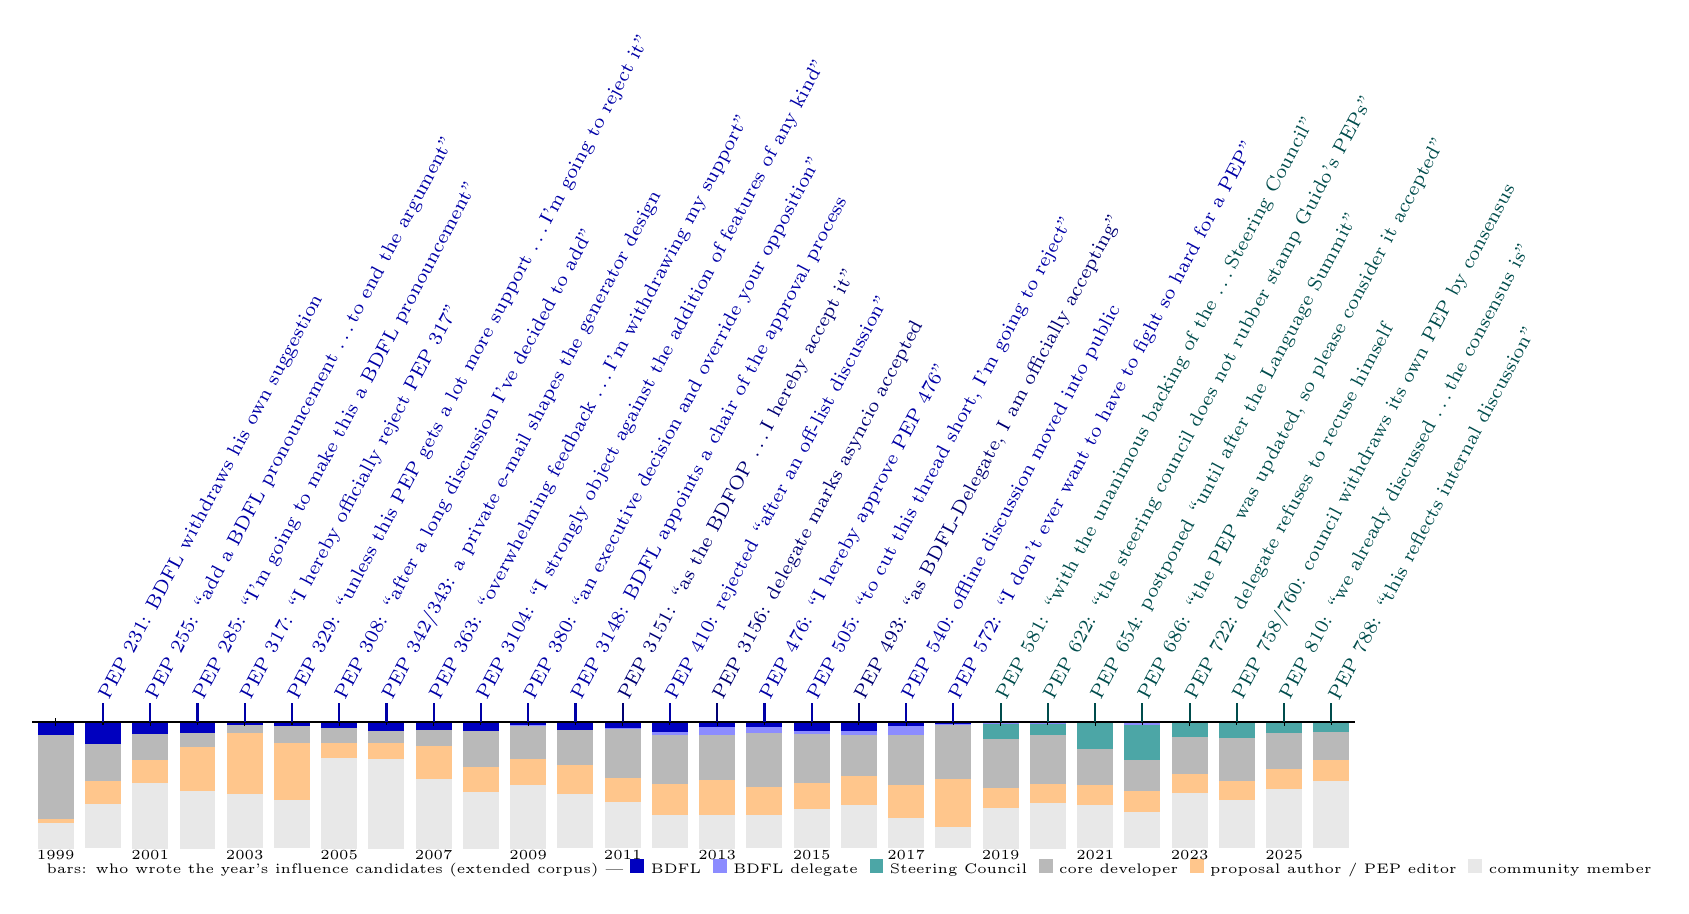
\begin{tikzpicture}[x=0.6cm, y=1cm, font=\scriptsize]
  % ---- stacked role shares of the year's influence candidates (extended corpus) ----
  % order (bottom to top): BDFL, BDFL delegate, steering council, core developer, author+editor, community
  \foreach \yr/\a/\b/\c/\d/\e/\f in {
    1999/10.0/0.0/0.0/66.3/3.8/20.0, 2000/17.2/0.0/0.0/29.2/18.4/35.2, 2001/9.2/0.0/0.0/20.9/17.9/52.1,
    2002/8.4/0.0/0.0/11.2/35.1/45.4, 2003/1.7/0.0/0.0/6.9/48.3/43.1, 2004/2.7/0.0/0.0/13.4/45.8/38.1,
    2005/4.4/0.0/0.0/11.6/12.5/71.6, 2006/6.8/0.0/0.0/9.3/12.9/71.1, 2007/6.2/0.0/0.0/12.9/26.0/55.0,
    2008/7.0/0.0/0.0/28.4/19.7/45.0, 2009/2.1/0.6/0.0/26.7/20.2/50.5, 2010/6.0/0.0/0.0/27.6/23.5/42.9,
    2011/4.2/1.2/0.0/38.8/19.0/36.8, 2012/7.5/2.4/0.0/38.7/25.0/26.3, 2013/3.9/6.1/0.0/35.7/27.7/26.7,
    2014/3.5/5.1/0.0/42.4/22.8/26.1, 2015/6.6/2.8/0.0/38.8/20.3/31.5, 2016/7.2/2.7/0.0/32.6/23.2/34.3,
    2017/3.2/7.1/0.0/39.2/26.0/24.3, 2018/1.6/0.7/0.0/42.7/37.7/16.7, 2019/0.0/1.4/11.5/38.9/16.2/32.1,
    2020/0.0/1.5/8.6/38.9/15.0/36.1, 2021/0.0/0.2/20.8/28.6/16.3/34.0, 2022/0.0/1.7/28.0/24.4/16.8/29.1,
    2023/0.0/0.4/11.3/29.4/15.2/43.7, 2024/0.0/0.2/12.1/34.5/15.0/38.2, 2025/0.0/0.6/7.8/29.0/15.1/47.5,
    2026/0.0/0.4/7.6/22.2/16.4/53.4} {
    \pgfmathsetmacro{\xl}{\yr-1999+0.12}
    \pgfmathsetmacro{\xr}{\yr-1999+0.88}
    \pgfmathsetmacro{\ya}{-\a*0.016}
    \pgfmathsetmacro{\yb}{\ya-\b*0.016}
    \pgfmathsetmacro{\yc}{\yb-\c*0.016}
    \pgfmathsetmacro{\yd}{\yc-\d*0.016}
    \pgfmathsetmacro{\ye}{\yd-\e*0.016}
    \pgfmathsetmacro{\yf}{\ye-\f*0.016}
    \fill[blue!75!black] (\xl,0) rectangle (\xr,\ya);
    \fill[blue!45] (\xl,\ya) rectangle (\xr,\yb);
    \fill[teal!70] (\xl,\yb) rectangle (\xr,\yc);
    \fill[gray!55] (\xl,\yc) rectangle (\xr,\yd);
    \fill[orange!45] (\xl,\yd) rectangle (\xr,\ye);
    \fill[gray!18] (\xl,\ye) rectangle (\xr,\yf);
  }
  \node[anchor=west, font=\tiny, align=left] at (0.1,-1.85) {bars: who wrote the year's influence candidates (extended corpus) ---
    \textcolor{blue!75!black}{\rule{5pt}{5pt}} BDFL\;
    \textcolor{blue!45}{\rule{5pt}{5pt}} BDFL delegate\;
    \textcolor{teal!70}{\rule{5pt}{5pt}} Steering Council\;
    \textcolor{gray!55}{\rule{5pt}{5pt}} core developer\;
    \textcolor{orange!45}{\rule{5pt}{5pt}} proposal author / PEP editor\;
    \textcolor{gray!18}{\rule{5pt}{5pt}} community member};
  % ---- axis and years ----
  \draw[thick] (0,0) -- (28,0);
  \foreach \yr in {1999,2001,...,2025} {
    \draw (\yr-1999+0.5,0.05) -- (\yr-1999+0.5,-0.05);
    \node[font=\tiny] at (\yr-1999+0.5,-1.68) {\yr};
  }
  \foreach \yr in {2000,2002,...,2026} { \draw (\yr-1999+0.5,0.03) -- (\yr-1999+0.5,-0.03); }
  % ---- one landmark influence act per year, nominated by the tool (Table tab:landmarks) ----
  \tikzset{bdfl/.style={blue!65!black}, dele/.style={blue!45!black}, sc/.style={teal!60!black}}
  \foreach \yr/\c/\t in {
    2000/bdfl/{PEP 231: BDFL withdraws his own suggestion},
    2001/bdfl/{PEP 255: ``add a BDFL pronouncement \ldots to end the argument''},
    2002/bdfl/{PEP 285: ``I'm going to make this a BDFL pronouncement''},
    2003/bdfl/{PEP 317: ``I hereby officially reject PEP 317''},
    2004/bdfl/{PEP 329: ``unless this PEP gets a lot more support \ldots I'm going to reject it''},
    2005/bdfl/{PEP 308: ``after a long discussion I've decided to add''},
    2006/bdfl/{PEP 342/343: a private e-mail shapes the generator design},
    2007/bdfl/{PEP 363: ``overwhelming feedback \ldots I'm withdrawing my support''},
    2008/bdfl/{PEP 3104: ``I strongly object against the addition of features of any kind''},
    2009/bdfl/{PEP 380: ``an executive decision and override your opposition''},
    2010/bdfl/{PEP 3148: BDFL appoints a chair of the approval process},
    2011/dele/{PEP 3151: ``as the BDFOP \ldots I hereby accept it''},
    2012/bdfl/{PEP 410: rejected ``after an off-list discussion''},
    2013/dele/{PEP 3156: delegate marks asyncio accepted},
    2014/bdfl/{PEP 476: ``I hereby approve PEP 476''},
    2015/bdfl/{PEP 505: ``to cut this thread short, I'm going to reject''},
    2016/dele/{PEP 493: ``as BDFL-Delegate, I am officially accepting''},
    2017/bdfl/{PEP 540: offline discussion moved into public},
    2018/bdfl/{PEP 572: ``I don't ever want to have to fight so hard for a PEP''},
    2019/sc/{PEP 581: ``with the unanimous backing of the \ldots Steering Council''},
    2020/sc/{PEP 622: ``the steering council does not rubber stamp Guido's PEPs''},
    2021/sc/{PEP 654: postponed ``until after the Language Summit''},
    2022/sc/{PEP 686: ``the PEP was updated, so please consider it accepted''},
    2023/sc/{PEP 722: delegate refuses to recuse himself},
    2024/sc/{PEP 758/760: council withdraws its own PEP by consensus},
    2025/sc/{PEP 810: ``we already discussed \ldots the consensus is''},
    2026/sc/{PEP 788: ``this reflects internal discussion''}} {
    \draw[\c, thick] (\yr-1999+0.5,0) -- (\yr-1999+0.5,0.25);
    \node[\c, rotate=62, anchor=west, inner sep=1pt] at (\yr-1999+0.5,0.27) {\t};
  }
\end{tikzpicture}
\caption{Landmark influence acts nominated by Influence Miner, 2000--2026: for each year, the highest-scoring sentence by a decision-maker of the time that carries a decision-closing mechanism (unilateral, gatekeeping, exit threat or backchannel), coloured by the author's role (dark blue: the BDFL; mid blue: a BDFL delegate; teal: a Steering Council member); full sentences in Table~\ref{tab:landmarks}. Below the axis, the share of each year's influence candidates written by each role. The sequence runs from personal pronouncements (2001--2009) through delegation (2010--2017) to the council's formulas of collective and procedural decision (2019--2026).}
\label{fig:timeline2}
\Description{A horizontal timeline from 1999 to 2026 with one short quoted sentence per year rising from the axis at an angle, coloured by whether the BDFL, a delegate or a Steering Council member wrote it, and stacked bars below the axis showing the share of influence candidates written by each role per year; the BDFL's share shrinks over time and the Steering Council's appears from 2019.}
\end{figure*}

\begin{table*}[t]
\caption{The landmark influence acts of Figure~\ref{fig:timeline2}: for each year, the highest-scoring decision-closing sentence by a decision-maker of the time in the extended corpus (score in brackets; mechanisms as labelled by the tool).}
\label{tab:landmarks}
\footnotesize
\begin{tabular}{p{0.03\textwidth}p{0.04\textwidth}p{0.14\textwidth}p{0.11\textwidth}p{0.60\textwidth}}
\toprule
Year & PEP & Author (role) & Mechanisms & Sentence \\
\midrule
2000 & 231 & van Rossum (BDFL) & exit threat & I withdraw the suggestion, and propose restricted execution instead. [2.6] \\
2001 & 255 & van Rossum (BDFL) & authority, unilateral & Tim, please add a BDFL pronouncement to the PEP to end the argument. [3.2] \\
2002 & 285 & van Rossum (BDFL) & authority, unilateral & I'm going to make this a BDFL pronouncement; I understand your argument but I don't agree with it. [4.3] \\
2003 & 317 & van Rossum (BDFL) & unilateral & I hereby officially reject PEP 317. [4.2] \\
2004 & 329 & van Rossum (BDFL) & unilateral & Also, a heads up: unless this PEP gets a lot more support from folks whose first name isn't Raymond, I'm going to reject it. [4.6] \\
2005 & 308 & van Rossum (BDFL) & compatibility, unilateral & After a long discussion I've decided to add a shortcut conditional expression to Python 2.5. [3.7] \\
2006 & 343 & van Rossum (BDFL) & backchannel & Bram Cohen pointed out in private email that, before PEP 342, there wasn't a big need for a shortcut to pass control to a ``sub-generator'' \ldots [3.7] \\
2007 & 363 & van Rossum (BDFL) & coalition, exit threat & This seems to be the overwhelming feedback at this point, so I'm withdrawing my support for the proposal. [4.4] \\
2008 & 3104 & van Rossum (BDFL) & operational, gatekeeping & I strongly object against the addition of features of *any* kind to 3.0.1, no matter whether they were promised or announced in a PEP or in the docs or on the 8 o'clock news. [4.0] \\
2009 & 380 & van Rossum (BDFL) & unilateral & Well, after thinking about it some more I think I am going to have to take an executive decision and override your opposition. :-) [2.6] \\
2010 & 3148 & van Rossum (BDFL) & unilateral & Since I really don't have the time or expertise to make a judgment on this PEP, I hereby appoint you chair of the approval process for this PEP. [3.6] \\
2011 & 3151 & Warsaw (delegate) & compatibility, unilateral & As the BDFOP for PEP 3151, I hereby accept it for inclusion into Python 3.3. [4.3] \\
2012 & 410 & van Rossum (BDFL) & authority, unilateral, backchannel & After an off-list discussion with Victor I have decided to reject PEP 410. [4.6] \\
2013 & 3156 & Pitrou (delegate) & authority, unilateral & I have decided to mark PEP 3156 accepted. [2.9] \\
2014 & 476 & van Rossum (BDFL) & unilateral & I see no reason to hold up this PEP's approval any longer, so I hereby approve PEP 476. [4.0] \\
2015 & 505 & van Rossum (BDFL) & unilateral & Just to cut this thread short, I'm going to reject PEP 505, because ? is just too ugly to add to Python IMO. [4.2] \\
2016 & 493 & Warsaw (delegate) & authority, unilateral & As BDFL-Delegate, I am officially accepting PEP 493. [2.9] \\
2017 & 540 & van Rossum (BDFL) & backchannel & I've been discussing this PEP offline with Victor, but he suggested we should discuss it in public instead. [4.2] \\
2018 & 572 & van Rossum (BDFL) & coalition, exit threat & Now that PEP 572 is done, I don't ever want to have to fight so hard for a PEP and find that so many people despise my decisions. [4.4] \\
2019 & 581 & Warsaw (SC) & authority, coalition, unilateral & As the BDFL-Delegate for PEP 581, and with the unanimous backing of the rest of the Steering Council, I hereby Accept this PEP. [4.6] \\
2020 & 622 & Cannon (SC) & authority, incivility, backchannel & I'm trying to not take that as an insult, but I will say the steering council does not rubber stamp Guido's PEPs. [2.7] \\
2021 & 654 & Galindo Salgado (SC) & tactical, authority, backchannel & The Steering Council discussed PEP 654: Exception Groups and except* \ldots deciding to postpone the PEP to 3.11, and postpone their decision for 3.11 until after the Language Summit. [3.6] \\
2022 & 686 & Viktorin (SC) & unilateral & The PEP was updated, so please consider it accepted. [4.0] \\
2023 & 722 & Cannon (SC) & authority, exit threat & I will step down as PEP delegate if Paul asks me, but otherwise I disagree with your reasoning as to why I shouldn't be the PEP delegate in this situation, and so I have no plans to recuse myself. [4.2] \\
2024 & 758/760 & Galindo Salgado (SC) & economic, coalition, exit threat & Update: We have decided to withdraw the PEP as the consensus is that the benefits doesn't justify the cost. [3.6] \\
2025 & 810 & Galindo Salgado (SC) & coalition, backchannel, procedural & We already discussed some version of this early in the discussion and the consensus is that \texttt{mod.\_\_dict\_\_} should not reify. [3.5] \\
2026 & 788 & Na (SC) & operational, backchannel & This reflects internal discussion that, if the PEP is officially approved, the implementer should have enough time to proceed with the implementation before the beta cutoff (May 5). [4.1] \\
\bottomrule
\end{tabular}
\end{table*}

\section{Discussion}

\paragraph{What the mechanism profile says about Python.} Python's proposal discussions are dominated by operational, functional, ecosystem and compatibility arguments. Influence in a mature language community is exercised mainly by arguing about whether something can be implemented and maintained, whether it solves a real problem, what it does to the ecosystem and what it breaks---and the lifecycle profile shows these arguments arriving in that order. Explicit appeals to authority are comparatively rare (7\%) even though the BDFL is the single most active participant, which supports the position taken in Section~4 that authority should be measured by uptake rather than assumed from role.

\paragraph{Governance transition.} The era comparison is the first quantitative trace of the governance transition in the discussions themselves. The mechanisms the community uses barely changed; what changed is the decision-makers' share of the conversation and their register. A five-person council that must document, delegate and announce invokes authority four times as often as the BDFL did and argues about implementation and compatibility rather than design, while functional and strategic arguments moved to authors and the community. Whether this reflects the council's mandate (PEP~13 asks it to decide, not to design) or the maturity of the language is a question for the qualitative follow-up.

\paragraph{Controversial influence is rare, concentrated, and changes form.} One candidate sentence in twenty exercises influence in a way the governance literature treats as contested, and those sentences are not spread evenly: they pile up in the debates the community remembers as painful and in the days before a decision. That the transition to the Steering Council left the total unchanged but shifted it from persons to process---fewer decisions by fiat, less gatekeeping and less incivility; twice as much procedural control and more disclosure of corporate stakes---is the clearest evidence in this study that governance design changes \emph{how} influence is exercised even when it does not change what people argue about. It is also a warning about what a procedural regime looks like from the inside: the council's members are the least likely of any role to decide by fiat and the most likely to point at PEP~13, to report internal discussion, and to say who they work for.

\paragraph{Volume is not influence.} The near-base-rate alignment of stance sentences with outcomes is the most important methodological result. It shows that a decision-mining tool that counted supporting and blocking sentences would learn nothing about outcomes in this corpus. Influence Miner's value lies in the mechanisms, roles and timing attached to each sentence, which allow the analyst to ask \emph{which} objections were taken up and \emph{whose} arguments the final PEP text reflects.

\paragraph{Data quality as a research finding.} Two problems in the shared corpus (Section~\ref{sec:dataquality}) would have silently distorted every actor-level result. Neither is visible in sentence-level statistics; both became obvious the moment an actor table was produced. Tools that report who said what should always produce that table.

\paragraph{Towards Bitcoin.} The taxonomy already contains the Bitcoin vocabulary (soft/hard forks, miners, wallets, consensus failure, fee market), the outcome resolver accepts BIP statuses, and the message source discovers column names, so the pipeline can be pointed at the DeMaP Miner BIP database. The comparison will test the expectation that Bitcoin shows stronger ecosystem, economic, security and deployment-based influence and weaker internal role-based influence.

\begin{table*}[t]
\caption{Three consecutive rows of the PEP~572 discussion in \texttt{allmessages}: the address column belongs to the following row.}
\label{tab:shift}
\small
\begin{tabular}{llll}
\toprule
Message id & Address column & Clustered name & Raw \texttt{From:} header \\
\midrule
8182634 & chris.jerdonek@gmail.com & Chris Angelico & rosuav at gmail.com (Chris Angelico) \\
8182635 & rosuav@gmail.com & Chris Jerdonek & chris.jerdonek at gmail.com (Chris Jerdonek) \\
8182636 & ncoghlan@gmail.com & Chris Angelico & rosuav at gmail.com (Chris Angelico) \\
\bottomrule
\end{tabular}
\end{table*}
\section{Data-Quality Findings in the Shared Corpus}
\label{sec:dataquality}

Two properties of the \texttt{allmessages} table would have silently distorted every actor-level result of this study, and are likely to affect other tools built on the same corpus. Both were found by inspecting the actor tables of early runs, which is itself an argument for producing such tables.

\paragraph{Automated senders.} The table links 109,046 message rows to PEPs, but 28,412 of them are not discussion: commit notifications from \texttt{python-checkins} (each of which embeds the full text of the PEP being committed), bug- and patch-tracker robots (\texttt{report@\allowbreak bugs.python.org}, \texttt{status@\allowbreak bugs.python.org}, \texttt{noreply@\allowbreak sourceforge.net}) and similar. These rows are essential for DeMaP Miner's process mining, which reads state changes from commits, but they must be excluded from influence mining. The first full run that included them produced 565,952 candidates, and because every commit notification carries the shared address \texttt{python-checkins@python.org}, 307,000 of those candidates were credited to one committer. Influence Miner now skips a configurable list of senders and lists (28,412 rows; the batch log reports the count per proposal), and keys actors by the corpus's clustered display name rather than by address, which also merges a person's several addresses.

\paragraph{Shifted sender columns.} The rows imported by a newer loader---identifiable by a sender field of the form ``From \emph{localpart}''; 10,831 PEP-linked rows, mostly from 2017--2018 and including the whole PEP~572 discussion---carry the sender address of the \emph{next} row. Checked against the raw \texttt{From:} header stored with each message body, the clustered display name agrees with the header for 9,532 of the 10,831 rows and the address column for only 3,155; the role column, which the original tool derived from the name, is consistent with the name. Table~\ref{tab:shift} shows the pattern. An earlier version of Influence Miner assumed the opposite---that the address was right and the name shifted---and rebuilt names from addresses, which credited PEP~572's discussion to the wrong people (the top three ``participants'' were an occasional poster, a core developer and a PEP editor who had each written a fraction of the attributed sentences). The tool now keeps the name and role on such rows and parses the address from the raw header, and the corpus extension derives sender fields from the header for every new row, keyed by message id, so the shift cannot recur.


\paragraph{Duplicate message ids.} A message that mentions several PEPs is stored once per PEP with the same message id (109,046 PEP-linked rows, 91,562 distinct ids). This is by design, but sentence-level tools must collapse duplicates within a proposal, and any join on message id alone must also constrain the PEP.

\paragraph{Consequence for earlier results.} Rationale Miner and Preference Miner results built on the same rows are not affected in their sentence-level findings, but any actor- or role-level statistic computed from the 2017--2018 rows should be re-checked, and the automated senders should be excluded wherever sentence counts are interpreted as participation.

\section{Threats to Validity}
\label{sec:threats}

\paragraph{Construct validity.} The labels are produced by cue phrases and have not been validated against human judgement; precision and recall are unknown. Table~\ref{tab:samples} was chosen to show the mechanisms clearly, but the same extraction also produces clear errors: a BDFL sentence reporting broad support (``I haven't seen substantial opposition against the PEP \ldots many people have explicitly posted in support of it'') is labelled \emph{blocking} because of the word ``opposition''; ``Google should not [be] needed to find a PEP'' fires the \emph{organizational} cue on a company name used as a verb; any mention of PEP~8 fires \emph{standards}. The stratified annotation sample exported by the tool (top-scored, random, per-mechanism and per-outcome strata) is the instrument for the two-coder study that must precede any stronger claim. Multi-label counts overstate the number of distinct arguments. The controversial cues are more precision-oriented than the base cues but are still surface patterns: ``code of conduct'' and ``bikeshedding'' mark talk \emph{about} incivility as well as incivility, ``as BDFL-Delegate I hereby accept'' is a sanctioned pronouncement rather than a usurpation, and ``conflict of interest'' appears in election reports because none was found; three rounds of cue tightening on the full corpus removed the most frequent false positives (``I'll leave the details'', ``I designed'', ``won't happen until 3.5''), but the remaining labels index contested passages rather than establish abuse.

\paragraph{Internal validity.} Alignment between direction and outcome is descriptive association at sentence level; sentences from the same author and message are not independent, and no causal inference is attempted. A third of candidates post-date the recorded decision, so ``influence on the decision'' must be qualified by the decision phase, which the tool records.

\paragraph{Data quality.} The two corpus problems of Section~\ref{sec:dataquality} are corrected in the reported runs; the correction relies on the raw headers stored with each message, which the Discourse posts do not have (their usernames come from the API and are exact).

\paragraph{External validity.} RQ1, RQ2, RQ4 and RQ5 are reported on the 1999--2018 mailing-list corpus; RQ3 and RQ6 add the Steering Council era, whose discussions come partly from a different medium (Discourse threads, where usernames stand in for addresses and quoting conventions differ). Findings should not be generalised to projects with different governance structures until the Bitcoin comparison is done.

\paragraph{Role identification.} Roles are proposal-specific and partly time-sensitive (core developer and PEP editor appointment dates are used), but the corpus's own role labels are trusted where present; Steering Council membership is resolved by name and term, and Discourse participants are identified by username, so a person using different names on the two media would be counted twice.

\section{Conclusion}

This paper presented Influence Miner, a framework and implemented tool for mining influence mechanisms in OSS decision-making discussions, and its first application to the Python PEP corpus. Influence Miner extends DeMaP Miner, Rationale Miner and Preference Miner by classifying sentence-level influence signals into strategic, operational, functional, tactical, authority, compatibility, security, standards, ecosystem, economic, organizational, coalition and user-demand mechanisms, and by attaching direction, scope, target, role, outcome and timing to each signal. Across 523 PEPs and 80,634 messages, operational, functional, ecosystem and compatibility mechanisms dominate; functional and strategic arguments come first and compatibility and operational arguments follow the decision; signalling peaks in the four weeks around the decision; after the 2018 governance transition the mechanisms barely change but the Steering Council becomes a larger and more authority-invoking presence than the BDFL was; rejected proposals remain contested on functional and authority grounds while accepted ones move to compatibility and implementation; stance volume does not track outcomes; influence and preference signals occupy largely different sentences; and the seven controversial mechanisms, present in one candidate in twenty, concentrate in the community's bitterest debates and shift from decisions by persons to control by process after the governance transition. The next steps are the two-coder annotation study that the tool's sampler supports, replacement of the cue rules by validated classifiers, reply-uptake and revision-linkage features, a qualitative reading of the Steering Council era, and the Bitcoin comparison for which the pipeline is prepared.

\appendix

\section{Detector Rules}
\label{app:rules}

The rules are reproduced here so that the labels in this paper can be reproduced and criticised. All cues are matched case-insensitively on word boundaries; British and American spellings are both listed.

\paragraph{Mechanism cues (selection).} Table~\ref{tab:cues} lists representative cues per mechanism; the complete lists (about 60 cues per mechanism) are in \texttt{InfluenceTypeDetector.java}. Some broad words count only near a disambiguating word within 60 characters: \emph{break/breaks/broken} near \emph{compatib-, existing, code, API, user, change, backward}; \emph{risk} near \emph{security, attack, regression, break, compat, data, safety}; \emph{team} near \emph{release, core, dev, steering, security}; \emph{node(s)} near \emph{old, full, network, bitcoin, upgrade}; \emph{market} near \emph{fee, share, economic, incentive}; \emph{patch(es)} near \emph{submit, review, apply, reference, implement}; \emph{editor(s)} near \emph{PEP, BIP}; \emph{data} near \emph{show, evidence, measure, benchmark}. The word \emph{safe} on its own is not a cue. The controversial mechanisms are matched the same way, and their broad cues also need context: ownership claims (\emph{I maintain, my module, as the maintainer}) count only near a refusal or decision word; \emph{no way, no chance, won't happen} only near a proposal or refusal word; \emph{offline, in person, at PyCon, at the sprint} only near a discussion or decision word; \emph{internally, secret} only near deliberation words; \emph{grant, contract, hired, full-time} only near employer or funding words; \emph{exhausted, tired of, step down, walk away, hiatus, retire} only in the first person or near a project word; \emph{angry, insane, flame, insult, hostile} only next to a person or tone word; \emph{procedure, belongs on, the archives, drop it, please stop} only near a process, list or thread word.

\begin{table*}[t]
\caption{Representative cue phrases per mechanism (base mechanisms above the rule, controversial mechanisms below).}
\label{tab:cues}
\small
\begin{tabular}{p{0.15\textwidth}p{0.81\textwidth}}
\toprule
Mechanism & Cues \\
\midrule
Strategic & long term, future direction, philosophy, principles, Zen of Python, pythonic, readability, simplicity, decentrali[s/z]ation, project values, governance \\
Operational & implement(ation), maintain(ance), release, migration, deploy(ment), test suite, documentation, backport, feature freeze, reference implementation, CPython \\
Functional & solves, use case, edge case, corner case, API, behavio[u]r, semantics, syntax, alternative design, better approach, what problem, special case \\
Tactical & to summari[s/z]e, let's decide, can we agree, compromise, reframe, narrow, clarify, evidence, defer, postpone, next step, rough consensus, separate PEP, straw poll \\
Authority & BDFL, steering council, delegate, core developer(s), committer, maintainer, BIP editor, release manager, pronounce(ment), veto, Guido, final decision \\
Compatibility & backward(s) compatib-, incompatible, breaking change, existing code/users, legacy, Python 2/3, 2to3, deprecat-, regression, soft/hard fork \\
Security & security, attack(er), vulnerab-, risk, unsafe, safety, privacy, robust(ness), denial of service, exploit, double spend, consensus failure, crash, data loss \\
Standards & standard(s), specification, spec, RFC, convention, interoperab-, compliance, PEP~8, style guide, de facto standard \\
Ecosystem & ecosystem, downstream, librar(y/ies), package(s), PyPI, stdlib, third-party, distros, wallet(s), exchange(s), miner(s), node(s), Lightning, full node \\
Economic & cost(s), expensive, funding, incentive(s), fee(s), fee market, business, commercial, budget, developer time, block reward, mempool \\
Organizational & company, foundation, PSF, organi[s/z]ation, working group, release team, committee, sponsor, employer, Google, Microsoft, Red Hat, Bitcoin Core \\
Coalition & several/many people, we all agree, consensus seems/is, broad support, multiple developers, as others have said, unanimous(ly), seconded, me too \\
User demand & users want/need, people keep asking, frequently requested, pain point, beginners, newcomers, students, real users, widely used, adoption \\
\midrule
Unilateral & I have decided, I'm going to reject/accept, I hereby, consider it accepted, end of discussion, not up for debate, overrule, by fiat, pull rank, already merged/committed, as BDFL, BDFL pronouncement, I get to decide, made up my mind \\
Corporate interest & my employer, my/our company, at work, at Google/Dropbox/Microsoft/Red Hat/\ldots, our production, our customers, paid to, funded by, sponsored by, commercial interest, business needs, conflict of interest, internal fork, enterprise users, my manager \\
Gatekeeping & I will not merge, I won't accept, not going to happen, over my dead body, I refuse, I will revert, I veto, I (strongly) object, not on my watch, as the maintainer, my approval, dead on arrival, won't fly, no chance, $-$1000, strong $-$1, the answer is no \\
Exit threat & I'll fork, fork CPython, leaving python-dev, I quit, I resign, step down, count me out, I give up, walk away, stop contributing/maintaining, withdraw the PEP, if this goes in, burned out, fed up, last straw, ultimatum, unsubscribe, mute this thread, fight so hard, out of energy \\
Incivility & stupid, idiot, ridiculous, absurd, nonsense, clueless, garbage, shut up, troll, flame war, you (clearly) don't understand, waste of time, bikeshedding, ad hominem, personal attack, insult, rude, hostile, toxic, condescending, arrogant, harassment, code of conduct, calm down, who cares \\
Backchannel & offline, off-list, privately, in private, behind closed doors, at the sprint, language summit, at PyCon, on IRC/Zulip/Discord, I talked to, Guido and I, Guido told me, already been decided, without discussion, without consulting, python-committers, done deal, rubber stamp, cabal, inner circle, out of band, lack of transparency \\
Procedural control & wrong list/venue, belongs on python-ideas, take it to, out of scope, scope creep, PEP~1 says, the PEP process, follow the process, proper channels, moderator, locking this thread, please stop, drop it, already discussed, dead horse, read the archives, needs a sponsor, write a PEP, too late for, after the freeze, PEP~13, formal vote \\
\bottomrule
\end{tabular}
\end{table*}

\paragraph{Direction.} A sentence is \emph{supporting} on an explicit support phrase or a positive vote (\emph{+1, +0.5} at a token boundary), \emph{blocking} on an explicit objection or a negative vote (\emph{$-$1}); negated phrases are resolved first (\emph{I don't object, no objection, not against, can live with} $\rightarrow$ supporting; \emph{don't support, not in favour, not convinced, don't see the need, not worth} $\rightarrow$ blocking); a sentence with both supporting and blocking cues is ambiguous and stays \emph{neutral}; hedged sentences (\emph{maybe, perhaps, not sure, I wonder}) and questions never become supporting or blocking and are demoted to \emph{revising} when they carry a stance cue; otherwise \emph{revising} on revision cues (\emph{revise, alternative, compromise, defer, postpone, clarify, narrow the scope, needs more work, more evidence, instead of, what about, I'd prefer, unless, provided that}) and \emph{neutral} by default.

\paragraph{Scope and target.} Scope is \emph{internal} when the author's resolved role is one of BDFL, steering council, delegate, proposal author, PEP/BIP editor, core developer, release manager or maintainer, or when the sentence names such actors; \emph{external} when the sentence names users, downstream projects, libraries, companies, wallets, exchanges, miners, standards bodies, educators, researchers or ``my employer''; \emph{mixed} when both apply. The role alone never makes a sentence external. Target is the first of governance, security, compatibility, implementation, ecosystem, users and proposal whose cue list matches.

\paragraph{Preprocessing.} Lines are dropped when they start with a quote marker, are ``On \ldots wrote:'' introductions, mail headers, forwarded-message markers, message-id or address debris, Gmail-style dated quote introductions, divider lines, signature blocks (from ``\texttt{--}'' or a closing word such as \emph{regards, cheers, thanks} to the end unless prose resumes), mailing-list footers, embedded PEP text (from a ``PEP: \emph{n}'' header block onward), code, diffs or tracebacks. URLs become \texttt{<URL>}. Sentences are split on terminal punctuation followed by whitespace with abbreviations, version numbers and proposal references protected; short vote lines are kept whole; sentences of fewer than three words (other than votes), more than 120 words, or mostly non-alphabetic characters are dropped; duplicates within a proposal are collapsed after lower-casing and removing punctuation.

\begin{thebibliography}{00}

\bibitem{pep1}
Python Software Foundation. 2026. PEP 1 -- PEP Purpose and Guidelines. Retrieved September 12, 2026 from \url{https://peps.python.org/pep-0001/}

\bibitem{pep13}
Python Software Foundation. 2026. PEP 13 -- Python Language Governance. Retrieved September 12, 2026 from \url{https://peps.python.org/pep-0013/}

\bibitem{bitcoinbips}
Bitcoin Core Contributors. 2026. Bitcoin Improvement Proposals repository. Retrieved September 12, 2026 from \url{https://github.com/bitcoin/bips}

\bibitem{bip3}
Bitcoin Core Contributors. 2026. BIP 3 -- Updated BIP Process. Retrieved September 12, 2026 from \url{https://github.com/bitcoin/bips/blob/master/bip-0003.md}

\bibitem{sharma2021rationale}
Pankajeshwara Nand Sharma, Bastin Tony Roy Savarimuthu, and Nigel Stanger. 2021. Extracting Rationale for Open Source Software Development Decisions -- A Study of Python Email Archives. \emph{arXiv:2102.05232}. \url{https://arxiv.org/abs/2102.05232}

\bibitem{sharma2024rationale}
Pankajeshwara Nand Sharma, Bastin Tony Roy Savarimuthu, and Nigel Stanger. 2024. How are decisions made in open source software communities? Uncovering rationale from Python email repositories. \emph{Journal of Software: Evolution and Process}. \url{https://doi.org/10.1002/smr.2526}

\bibitem{sharma2021roles}
Pankajeshwara Nand Sharma, Bastin Tony Roy Savarimuthu, and Nigel Stanger. 2021. Influence of Roles in Decision-Making during OSS Development -- A Study of Python. \emph{arXiv:2106.02209}. \url{https://arxiv.org/abs/2106.02209}

\bibitem{sharma2022demap}
Pankajeshwara Nand Sharma, Bastin Tony Roy Savarimuthu, and Nigel Stanger. 2022. Unearthing open source decision-making processes: A case study of Python Enhancement Proposals. \emph{Software: Practice and Experience}. \url{https://doi.org/10.1002/spe.3128}

\bibitem{thapa2021bitcoin}
Rewat Thapa, Pankajeshwara Sharma, Joschka Andreas H{\"u}llmann, and Bastin Tony Roy Savarimuthu. 2021. Identifying Influence Mechanisms in Permissionless Blockchain Communities: The Bitcoin Case. In \emph{Proceedings of the 42nd International Conference on Information Systems (ICIS 2021)}, 1--17.

\bibitem{rationaleDesign}
Antony Tang, Yan Jin, and Jun Han. 2007. A rationale-based architecture model for design traceability and reasoning. \emph{Journal of Systems and Software} 80, 6, 918--934.

\bibitem{argumentMining}
Raquel Mochales and Marie-Francine Moens. 2011. Argumentation mining. \emph{Artificial Intelligence and Law} 19, 1, 1--22.

\bibitem{raymond1999}
Eric S. Raymond. 1999. \emph{The Cathedral and the Bazaar: Musings on Linux and Open Source by an Accidental Revolutionary}. O'Reilly.

\bibitem{omahony2007}
Siobh\'an O'Mahony and Fabrizio Ferraro. 2007. The emergence of governance in an open source community. \emph{Academy of Management Journal} 50, 5, 1079--1106.

\bibitem{dahlander2005}
Linus Dahlander and Mats G. Magnusson. 2005. Relationships between open source software companies and communities: Observations from Nordic firms. \emph{Research Policy} 34, 4, 481--493.

\bibitem{riehle2007}
Dirk Riehle. 2007. The economic motivation of open source software: Stakeholder perspectives. \emph{IEEE Computer} 40, 4, 25--32.

\bibitem{zhang2020}
Yuxia Zhang, Minghui Zhou, Klaas-Jan Stol, Jianyu Wu, and Zhi Jin. 2020. How do companies collaborate in open source ecosystems? An empirical study of OpenStack. In \emph{Proceedings of the 42nd International Conference on Software Engineering (ICSE 2020)}, 1196--1208.

\bibitem{ducheneaut2005}
Nicolas Ducheneaut. 2005. Socialization in an open source software community: A socio-technical analysis. \emph{Computer Supported Cooperative Work} 14, 4, 323--368.

\bibitem{jensen2007}
Chris Jensen and Walt Scacchi. 2007. Role migration and advancement processes in OSSD projects: A comparative case study. In \emph{Proceedings of the 29th International Conference on Software Engineering (ICSE 2007)}, 364--374.

\bibitem{hirschman1970}
Albert O. Hirschman. 1970. \emph{Exit, Voice, and Loyalty: Responses to Decline in Firms, Organizations, and States}. Harvard University Press.

\bibitem{robles2012}
Gregorio Robles and Jes\'us M. Gonz\'alez-Barahona. 2012. A comprehensive study of software forks: Dates, reasons and outcomes. In \emph{Open Source Systems: Long-Term Sustainability (OSS 2012)}, IFIP AICT 378, 1--14.

\bibitem{gamalielsson2014}
Jonas Gamalielsson and Bj\"orn Lundell. 2014. Sustainability of open source software communities beyond a fork: How and why has the LibreOffice project evolved? \emph{Journal of Systems and Software} 89, 128--145.

\bibitem{raman2020}
Naveen Raman, Minxuan Cao, Yulia Tsvetkov, Christian K\"astner, and Bogdan Vasilescu. 2020. Stress and burnout in open source: Toward finding, understanding, and mitigating unhealthy interactions. In \emph{ICSE-NIER 2020}, 57--60.

\bibitem{ferreira2021}
Isabella Ferreira, Jinghui Cheng, Bram Adams, and Eirini Kalliamvakou. 2021. The ``shut the f**k up'' phenomenon: Characterizing incivility in open source code review discussions. \emph{Proceedings of the ACM on Human-Computer Interaction} 5, CSCW2, Article 353.

\bibitem{squire2015}
Megan Squire and Rebecca Gazda. 2015. FLOSS as a source for profanity and insults: Collecting the data. In \emph{Proceedings of the 48th Hawaii International Conference on System Sciences (HICSS 2015)}, 5290--5298.

\bibitem{schneider2016}
Daniel Schneider, Scott Spurlock, and Megan Squire. 2016. Differentiating communication styles of leaders on the Linux kernel mailing list. In \emph{Proceedings of the 12th International Symposium on Open Collaboration (OpenSym 2016)}, Article 2.

\bibitem{delaat2007}
Paul B. de Laat. 2007. Governance of open source software: State of the art. \emph{Journal of Management \& Governance} 11, 2, 165--177.

\bibitem{fitzgerald2006}
Brian Fitzgerald. 2006. The transformation of open source software. \emph{MIS Quarterly} 30, 3, 587--598.

\bibitem{transferofpower}
Guido van Rossum. 2018. Transfer of power. Message to python-committers, 12 July 2018. Retrieved September 12, 2026 from \url{https://mail.python.org/pipermail/python-committers/2018-July/005664.html}

\bibitem{mockus2002}
Audris Mockus, Roy T. Fielding, and James D. Herbsleb. 2002. Two case studies of open source software development: Apache and Mozilla. \emph{ACM Transactions on Software Engineering and Methodology} 11, 3, 309--346.

\bibitem{fielding1999}
Roy T. Fielding. 1999. Shared leadership in the Apache project. \emph{Communications of the ACM} 42, 4, 42--43.

\bibitem{crowston2005}
Kevin Crowston and James Howison. 2005. The social structure of free and open source software development. \emph{First Monday} 10, 2.

\bibitem{stewart2005}
Daniel Stewart. 2005. Social status in an open-source community. \emph{American Sociological Review} 70, 5, 823--842.

\bibitem{vonkrogh2003}
Georg von Krogh, Sebastian Spaeth, and Karim R. Lakhani. 2003. Community, joining, and specialization in open source software innovation: A case study. \emph{Research Policy} 32, 7, 1217--1241.

\bibitem{weber2004}
Steven Weber. 2004. \emph{The Success of Open Source}. Harvard University Press.

\bibitem{shah2006}
Sonali K. Shah. 2006. Motivation, governance, and the viability of hybrid forms in open source software development. \emph{Management Science} 52, 7, 1000--1014.

\bibitem{markus2007}
M. Lynne Markus. 2007. The governance of free/open source software projects: Monolithic, multidimensional, or configurational? \emph{Journal of Management \& Governance} 11, 2, 151--163.

\bibitem{dahlander2011}
Linus Dahlander and Siobh\'an O'Mahony. 2011. Progressing to the center: Coordinating project work. \emph{Organization Science} 22, 4, 961--979.

\bibitem{fleming2007}
Lee Fleming and David M. Waguespack. 2007. Brokerage, boundary spanning, and leadership in open innovation communities. \emph{Organization Science} 18, 2, 165--180.

\bibitem{shaikh2017}
Maha Shaikh and Ola Henfridsson. 2017. Governing open source software through coordination processes. \emph{Information and Organization} 27, 2, 116--135.

\bibitem{lindberg2016}
Aron Lindberg, Nicholas Berente, James Gaskin, and Kalle Lyytinen. 2016. Coordinating interdependencies in online communities: A study of an open source software project. \emph{Information Systems Research} 27, 4, 751--772.

\bibitem{howison2014}
James Howison and Kevin Crowston. 2014. Collaboration through open superposition: A theory of the open source way. \emph{MIS Quarterly} 38, 1, 29--50.

\bibitem{tsay2014}
Jason Tsay, Laura Dabbish, and James Herbsleb. 2014. Influence of social and technical factors for evaluating contribution in GitHub. In \emph{Proceedings of the 36th International Conference on Software Engineering (ICSE 2014)}, 356--366.

\bibitem{tsay2014b}
Jason Tsay, Laura Dabbish, and James Herbsleb. 2014. Let's talk about it: Evaluating contributions through discussion in GitHub. In \emph{Proceedings of the 22nd ACM SIGSOFT International Symposium on Foundations of Software Engineering (FSE 2014)}, 144--154.

\bibitem{marlow2013}
Jennifer Marlow, Laura Dabbish, and Jim Herbsleb. 2013. Impression formation in online peer production: Activity traces and personal profiles in GitHub. In \emph{Proceedings of the 2013 Conference on Computer Supported Cooperative Work (CSCW 2013)}, 117--128.

\bibitem{alami2020}
Adam Alami, Marisa Leavitt Cohn, and Andrzej W\k{a}sowski. 2020. How do FOSS communities decide to accept pull requests? In \emph{Proceedings of the 24th International Conference on Evaluation and Assessment in Software Engineering (EASE 2020)}, 220--229.

\bibitem{steinmacher2015}
Igor Steinmacher, Tayana Conte, Marco Aur\'elio Gerosa, and David Redmiles. 2015. Social barriers faced by newcomers placing their first contribution in open source software projects. In \emph{Proceedings of the 18th ACM Conference on Computer Supported Cooperative Work and Social Computing (CSCW 2015)}, 1379--1392.

\bibitem{dahlander2006}
Linus Dahlander and Martin W. Wallin. 2006. A man on the inside: Unlocking communities as complementary assets. \emph{Research Policy} 35, 8, 1243--1259.

\bibitem{schaarschmidt2015}
Mario Schaarschmidt, Gianfranco Walsh, and Harald F. O. von Kortzfleisch. 2015. How do firms influence open source software communities? A framework and empirical analysis of different governance modes. \emph{Information and Organization} 25, 2, 99--114.

\bibitem{riehle2014}
Dirk Riehle, Philipp Riemer, Carsten Kolassa, and Michael Schmidt. 2014. Paid vs.\ volunteer work in open source. In \emph{Proceedings of the 47th Hawaii International Conference on System Sciences (HICSS 2014)}, 3286--3295.

\bibitem{zhang2021}
Yuxia Zhang, Minghui Zhou, Audris Mockus, and Zhi Jin. 2021. Companies' participation in OSS development: An empirical study of OpenStack. \emph{IEEE Transactions on Software Engineering} 47, 10, 2242--2259.

\bibitem{zhang2022}
Yuxia Zhang, Klaas-Jan Stol, Hui Liu, and Minghui Zhou. 2022. Corporate dominance in open source ecosystems: A case study of OpenStack. In \emph{Proceedings of the 30th ACM Joint European Software Engineering Conference and Symposium on the Foundations of Software Engineering (ESEC/FSE 2022)}, 1048--1060.

\bibitem{butler2018}
Simon Butler, Jonas Gamalielsson, Bj\"orn Lundell, Christoffer Brax, Anders Mattsson, Tomas Gustavsson, Jonas Feist, Bengt Kvarnstr\"om, and Erik L\"onroth. 2018. An investigation of work practices used by companies making contributions to established OSS projects. In \emph{Proceedings of the 40th International Conference on Software Engineering: Software Engineering in Practice (ICSE-SEIP 2018)}, 201--210.

\bibitem{elliott2003}
Margaret S. Elliott and Walt Scacchi. 2003. Free software developers as an occupational community: Resolving conflicts and fostering collaboration. In \emph{Proceedings of the 2003 International ACM SIGGROUP Conference on Supporting Group Work (GROUP 2003)}, 21--30.

\bibitem{jensen2004}
Chris Jensen and Walt Scacchi. 2004. Collaboration, leadership, control, and conflict negotiation in the NetBeans.org community. In \emph{Proceedings of the 4th Workshop on Open Source Software Engineering (ICSE 2004)}, 48--52.

\bibitem{filippova2016}
Anna Filippova and Hichang Cho. 2016. The effects and antecedents of conflict in free and open source software development. In \emph{Proceedings of the 19th ACM Conference on Computer-Supported Cooperative Work and Social Computing (CSCW 2016)}, 705--716.

\bibitem{miller2022}
Courtney Miller, Sophie Cohen, Daniel Klug, Bogdan Vasilescu, and Christian K\"astner. 2022. ``Did you miss my comment or what?'' Understanding toxicity in open source discussions. In \emph{Proceedings of the 44th International Conference on Software Engineering (ICSE 2022)}, 710--722.

\bibitem{barcellini2008a}
Flore Barcellini, Fran\c{c}oise D\'etienne, and Jean-Marie Burkhardt. 2008. User and developer mediation in an open source software community: Boundary spanning through cross participation in online discussions. \emph{International Journal of Human-Computer Studies} 66, 7, 558--570.

\bibitem{barcellini2008b}
Flore Barcellini, Fran\c{c}oise D\'etienne, Jean-Marie Burkhardt, and Warren Sack. 2008. A socio-cognitive analysis of online design discussions in an open source software community. \emph{Interacting with Computers} 20, 1, 141--165.

\bibitem{sack2006}
Warren Sack, Fran\c{c}oise D\'etienne, Nicolas Ducheneaut, Jean-Marie Burkhardt, Dilan Mahendran, and Flore Barcellini. 2006. A methodological framework for socio-cognitive analyses of collaborative design of open source software. \emph{Computer Supported Cooperative Work} 15, 2--3, 229--250.

\bibitem{keertipati2016}
Smitha Keertipati, Sherlock A. Licorish, and Bastin Tony Roy Savarimuthu. 2016. Exploring decision-making processes in Python. In \emph{Proceedings of the 20th International Conference on Evaluation and Assessment in Software Engineering (EASE 2016)}, Article 43.

\bibitem{sharma2017}
Pankajeshwara Sharma, Bastin Tony Roy Savarimuthu, Nigel Stanger, Sherlock A. Licorish, and Austen Rainer. 2017. Investigating developers' email discussions during decision-making in Python language evolution. In \emph{Proceedings of the 21st International Conference on Evaluation and Assessment in Software Engineering (EASE 2017)}, 286--291.

\bibitem{ossGovernance}
Kevin Crowston, Kangning Wei, James Howison, and Andrea Wiggins. 2012. Free/Libre open-source software development: What we know and what we do not know. \emph{ACM Computing Surveys} 44, 2, Article 7.

\end{thebibliography}

\end{document}
